\section{Introduction}
Tout d'abord, nos plus grandes félicitations pour votre impressionnante
performance tout au long des qualifications et des épreuves régionales
de Prologin.
Vous avez surmonté de nombreux défis, des qualifications en ligne
aux demi-finales régionales, comprenant de nombreuses épreuves
algorithmiques et divers autres challenges.
Votre réussite témoigne de votre talent et de votre persévérance,
et nous vous souhaitons désormais la bienvenue à la toute dernière
étape de cette aventure~: la finale~!

\section{Objectif}
Lors d'une partie, deux joueurs s'affrontent en un contre un sur une carte
rectangulaire.
Les deux joueurs cherchent à maintenir le plus grand territoire possible
\footnote{Sauf quand ils ne veulent pas.}.
Pour aider les deux joueurs dans leur mission, ils peuvent capturer des
aigles capables de façonner la terre
\footnote{Sauf quand ils ne veulent pas.}.

\section{Carte}
La carte est une grille rectangulaire de
$\mathtt{largeur} \times \mathtt{hauteur}$ cases.
La $\mathtt{largeur}$ est comprise entre \texttt{LARGEUR\_MIN} et
\texttt{LARGEUR\_MAX} (inclus), et la $\mathtt{hauteur}$ est comprise
entre \texttt{HAUTEUR\_MIN} et \texttt{HAUTEUR\_MAX} (inclus).

Les dimensions exactes de la carte ne sont pas fixées, et peuvent dépendre de
la carte.

\begin{figure}[h]
    \centering
    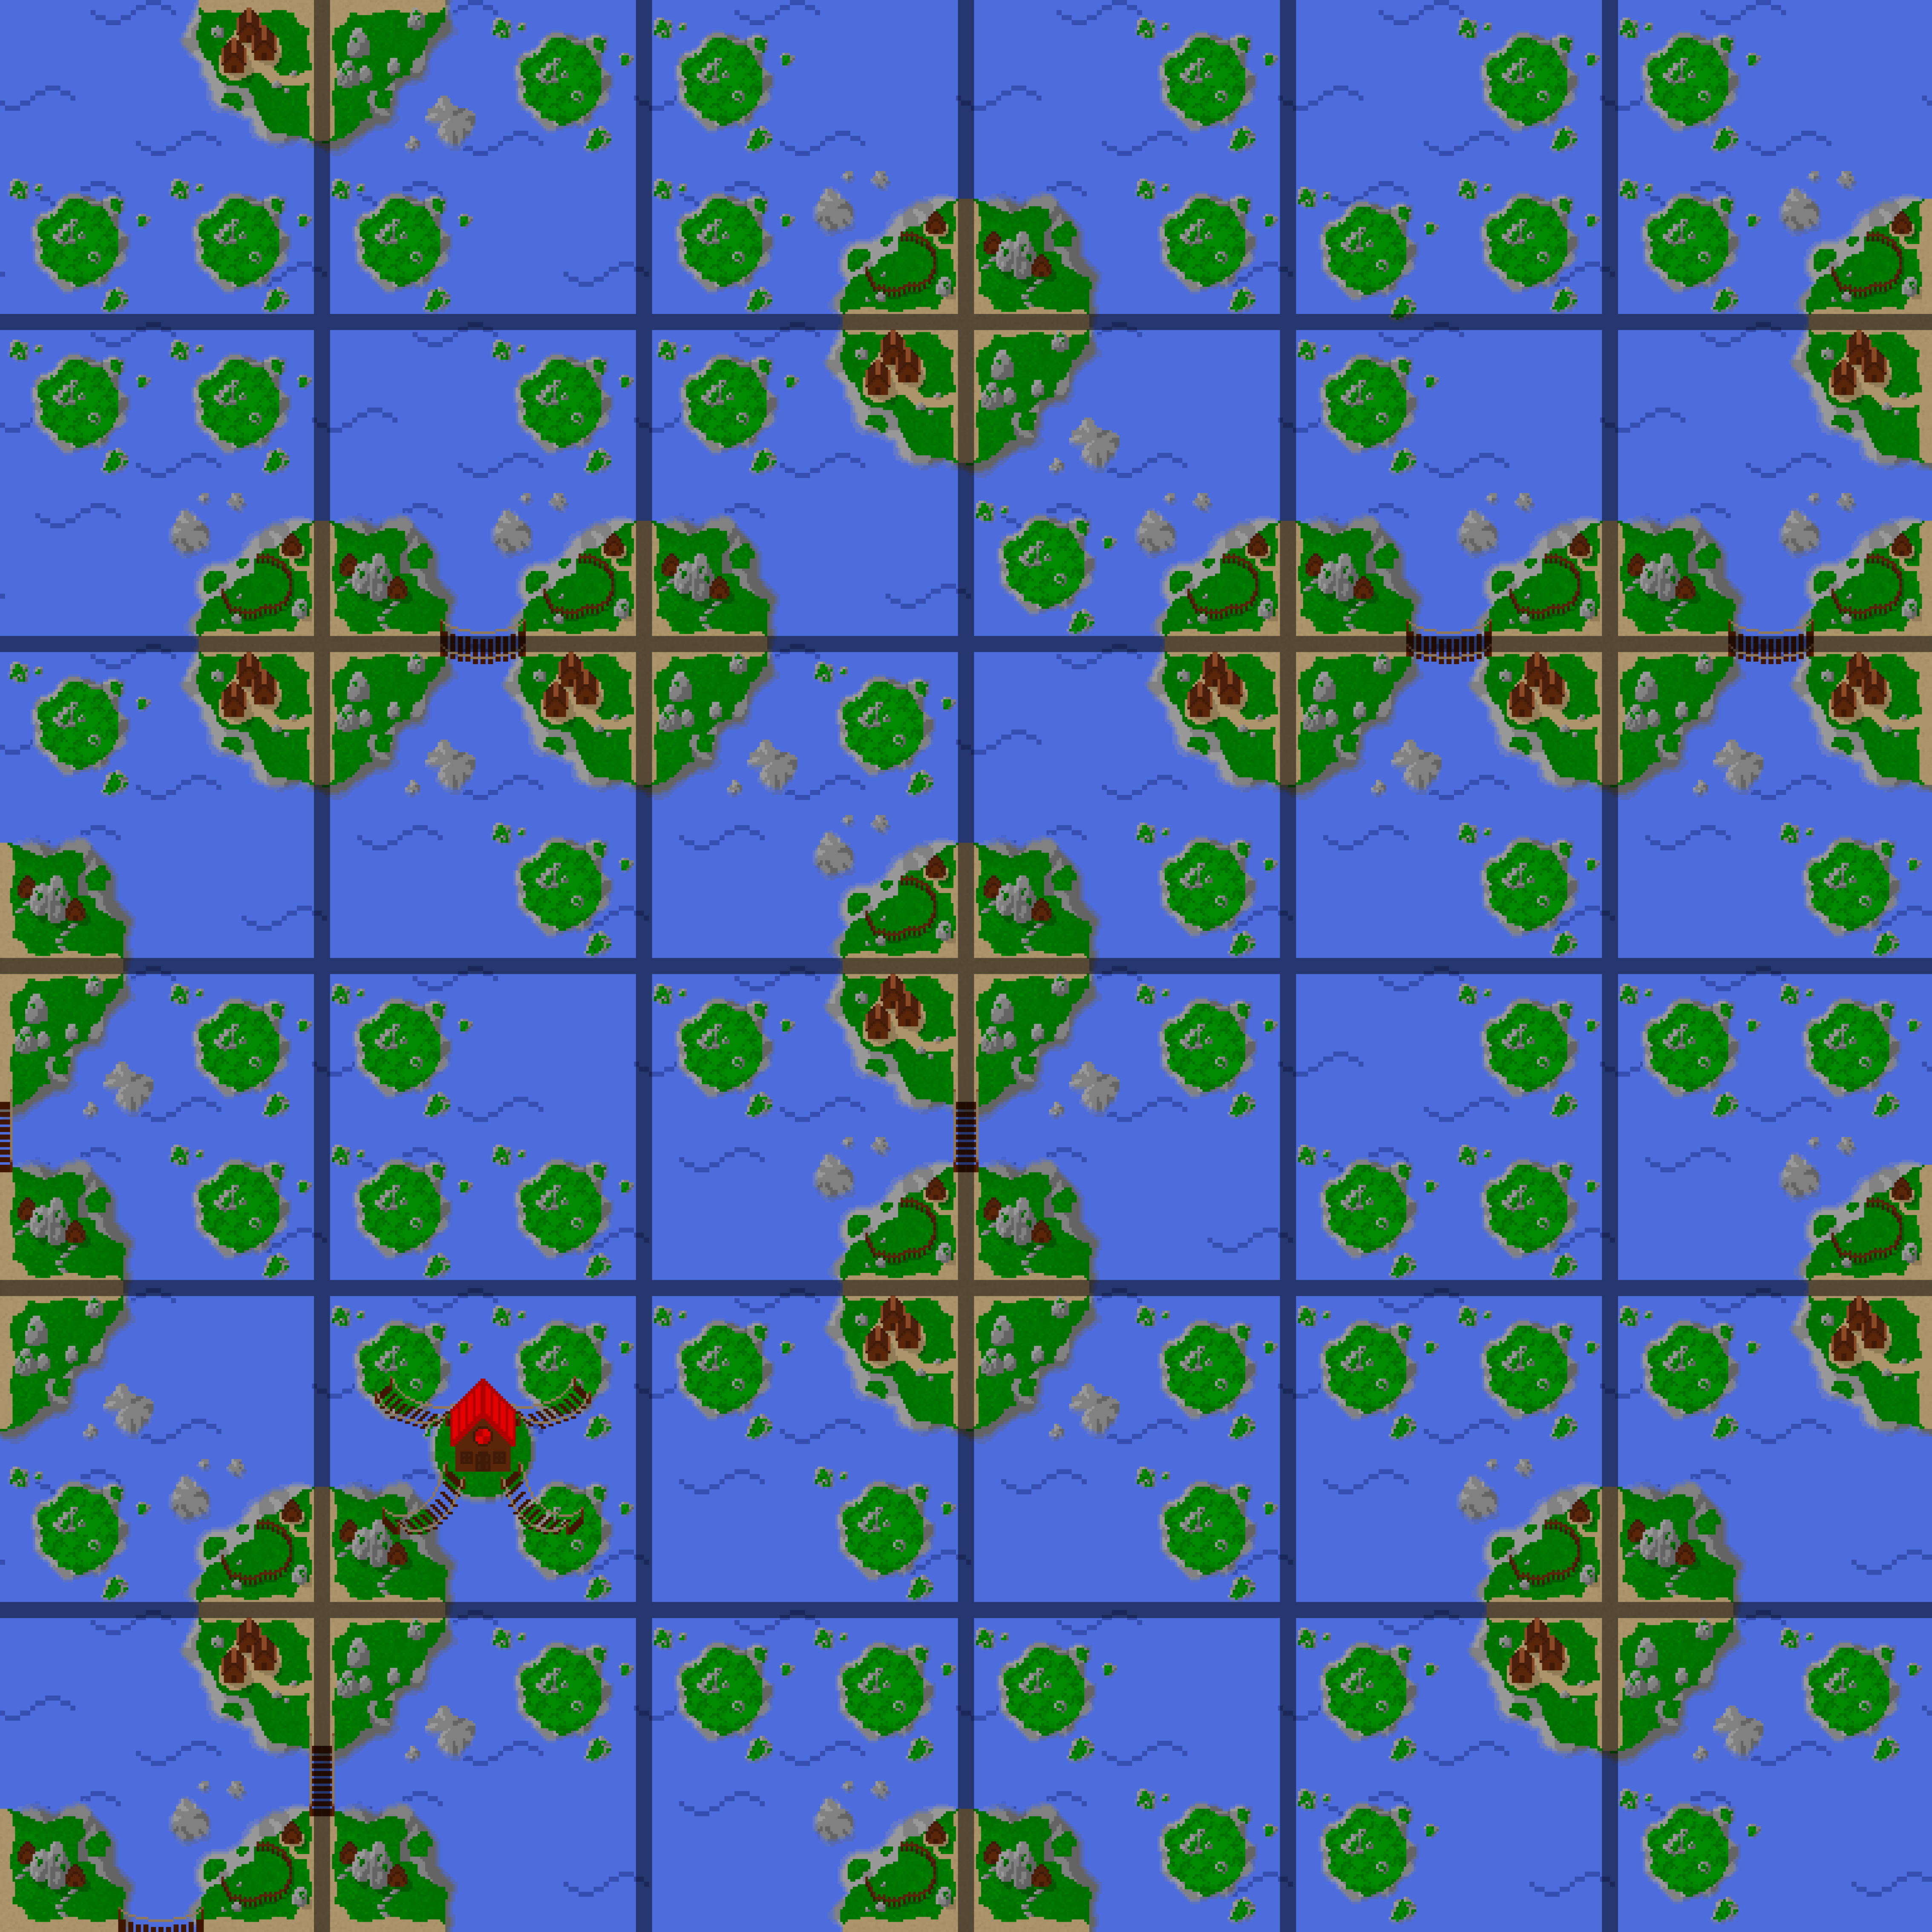
\includegraphics[width=0.4\textwidth]{img/sprites/carte.png}
    \caption{Exemple de carte de $6 \times 6$ cases}
\end{figure}

\subsection{Cases}
Les cases de la grille sont identifiées par leur position, un couple
$(\mathtt{colonne}, \mathtt{ligne})$, où la case dans le coin nord-ouest
possède la position $(0, 0)$, et la case dans le coin sud-est possède
la position $(\mathtt{largeur} - 1, \mathtt{hauteur} - 1)$.

\begin{figure}[h]
    \centering
    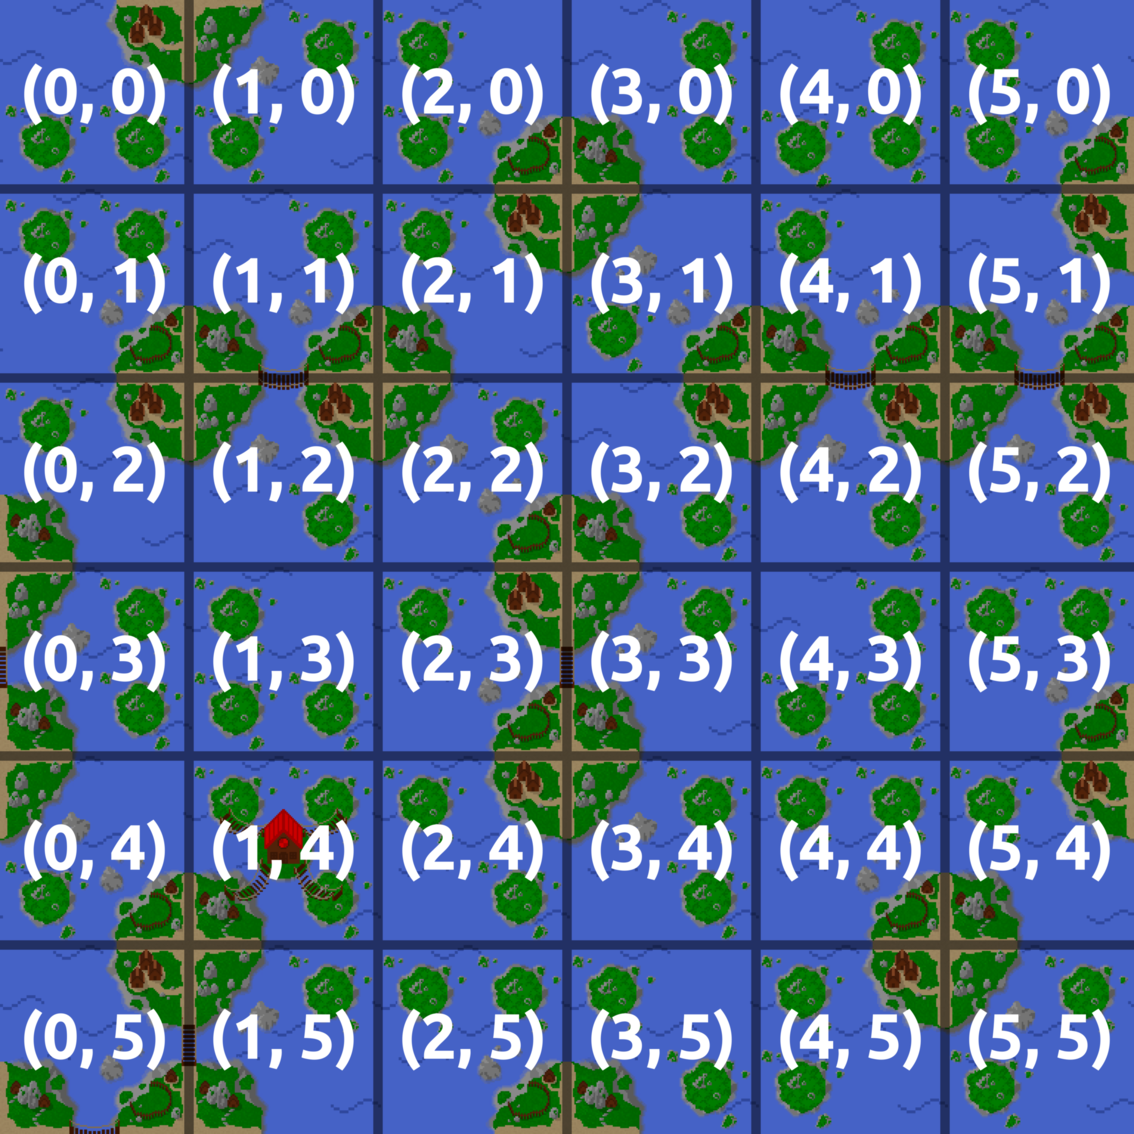
\includegraphics[width=0.5\textwidth]{img/sprites/cases.png}
    \caption{Coordonnées des cases de la carte}
\end{figure}

Une case peut contenir soit un village, soit trois îlots dans trois des quatre
coins de la case.
Une case contenant trois îlots est identifiée par le point cardinal
du coin ne possédant \textbf{pas} d'îlot. % footnote : point cardinal n'est pas évident et à reformuler.

La plupart des cases peuvent être tournées (Section \ref{sec:rotation}), à moins qu'elles ne soient gelées (Section \ref{sec:gel}).

\begin{figure}[h]
    \centering
    \begin{minipage}{0.23\textwidth}
        \centering
        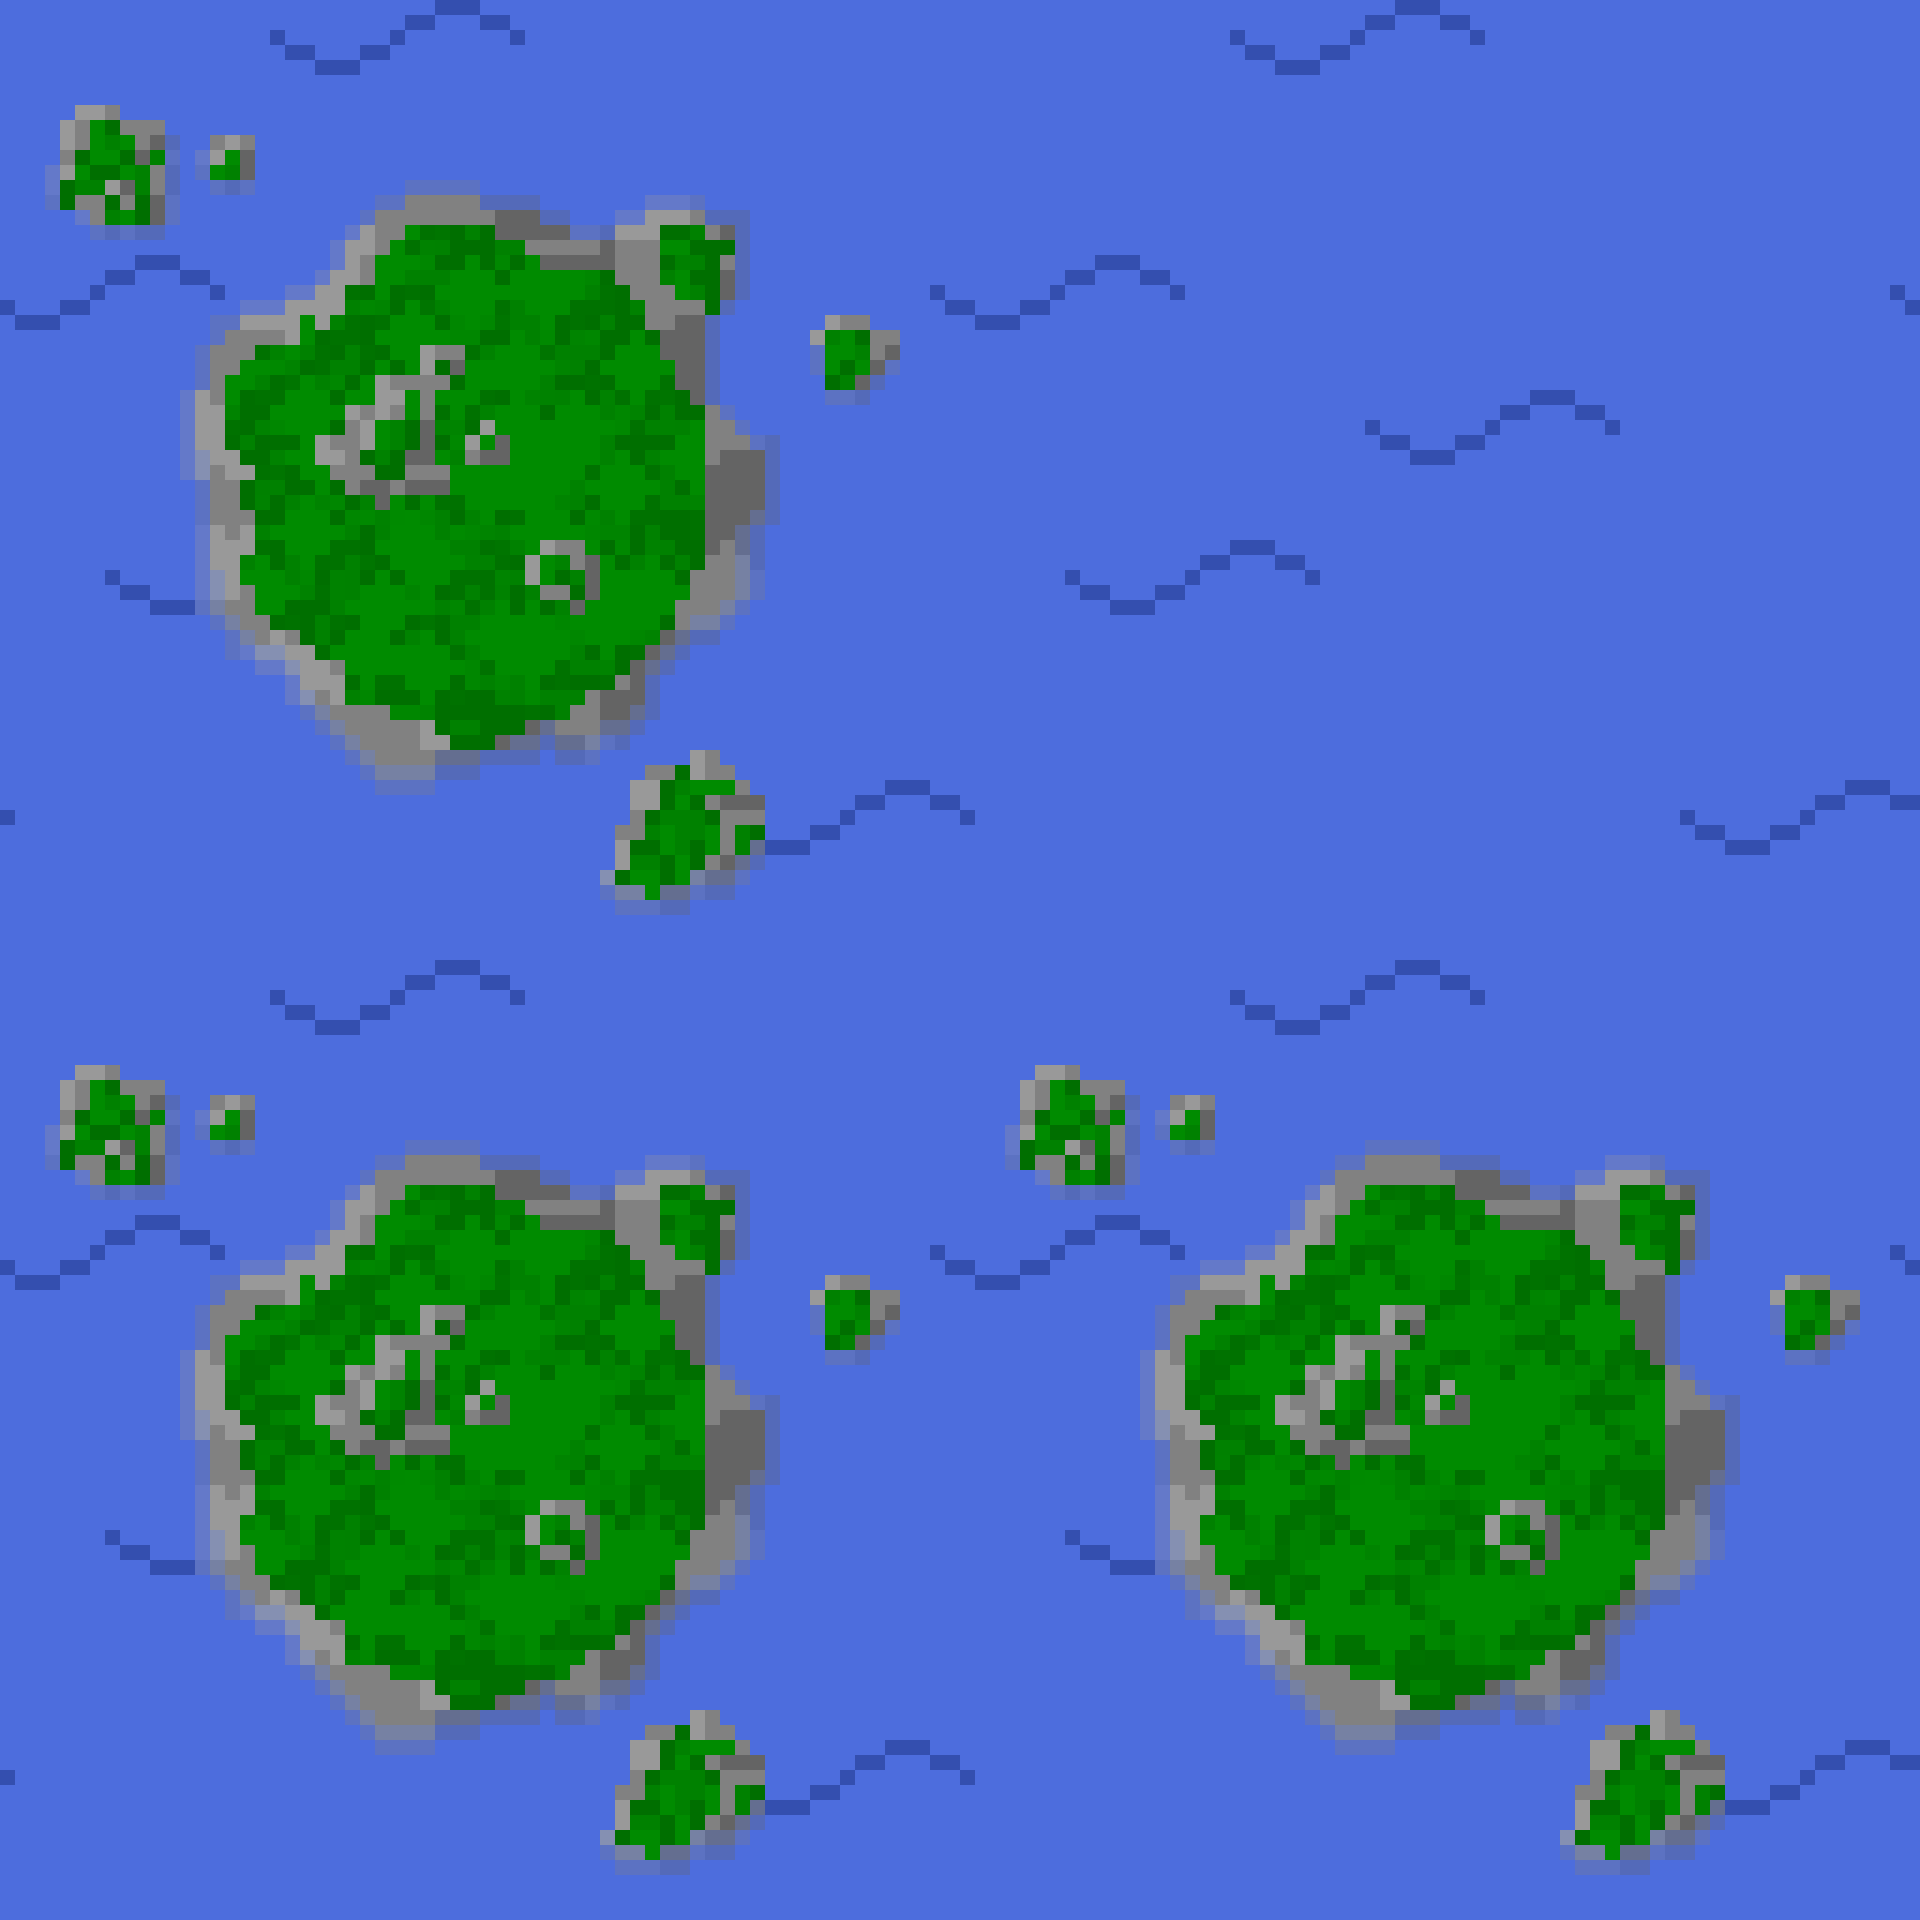
\includegraphics[width=0.8\textwidth]{img/sprites/1.png}
        \caption*{Case \texttt{NORD\_EST}}
    \end{minipage}
    \begin{minipage}{0.23\textwidth}
        \centering
        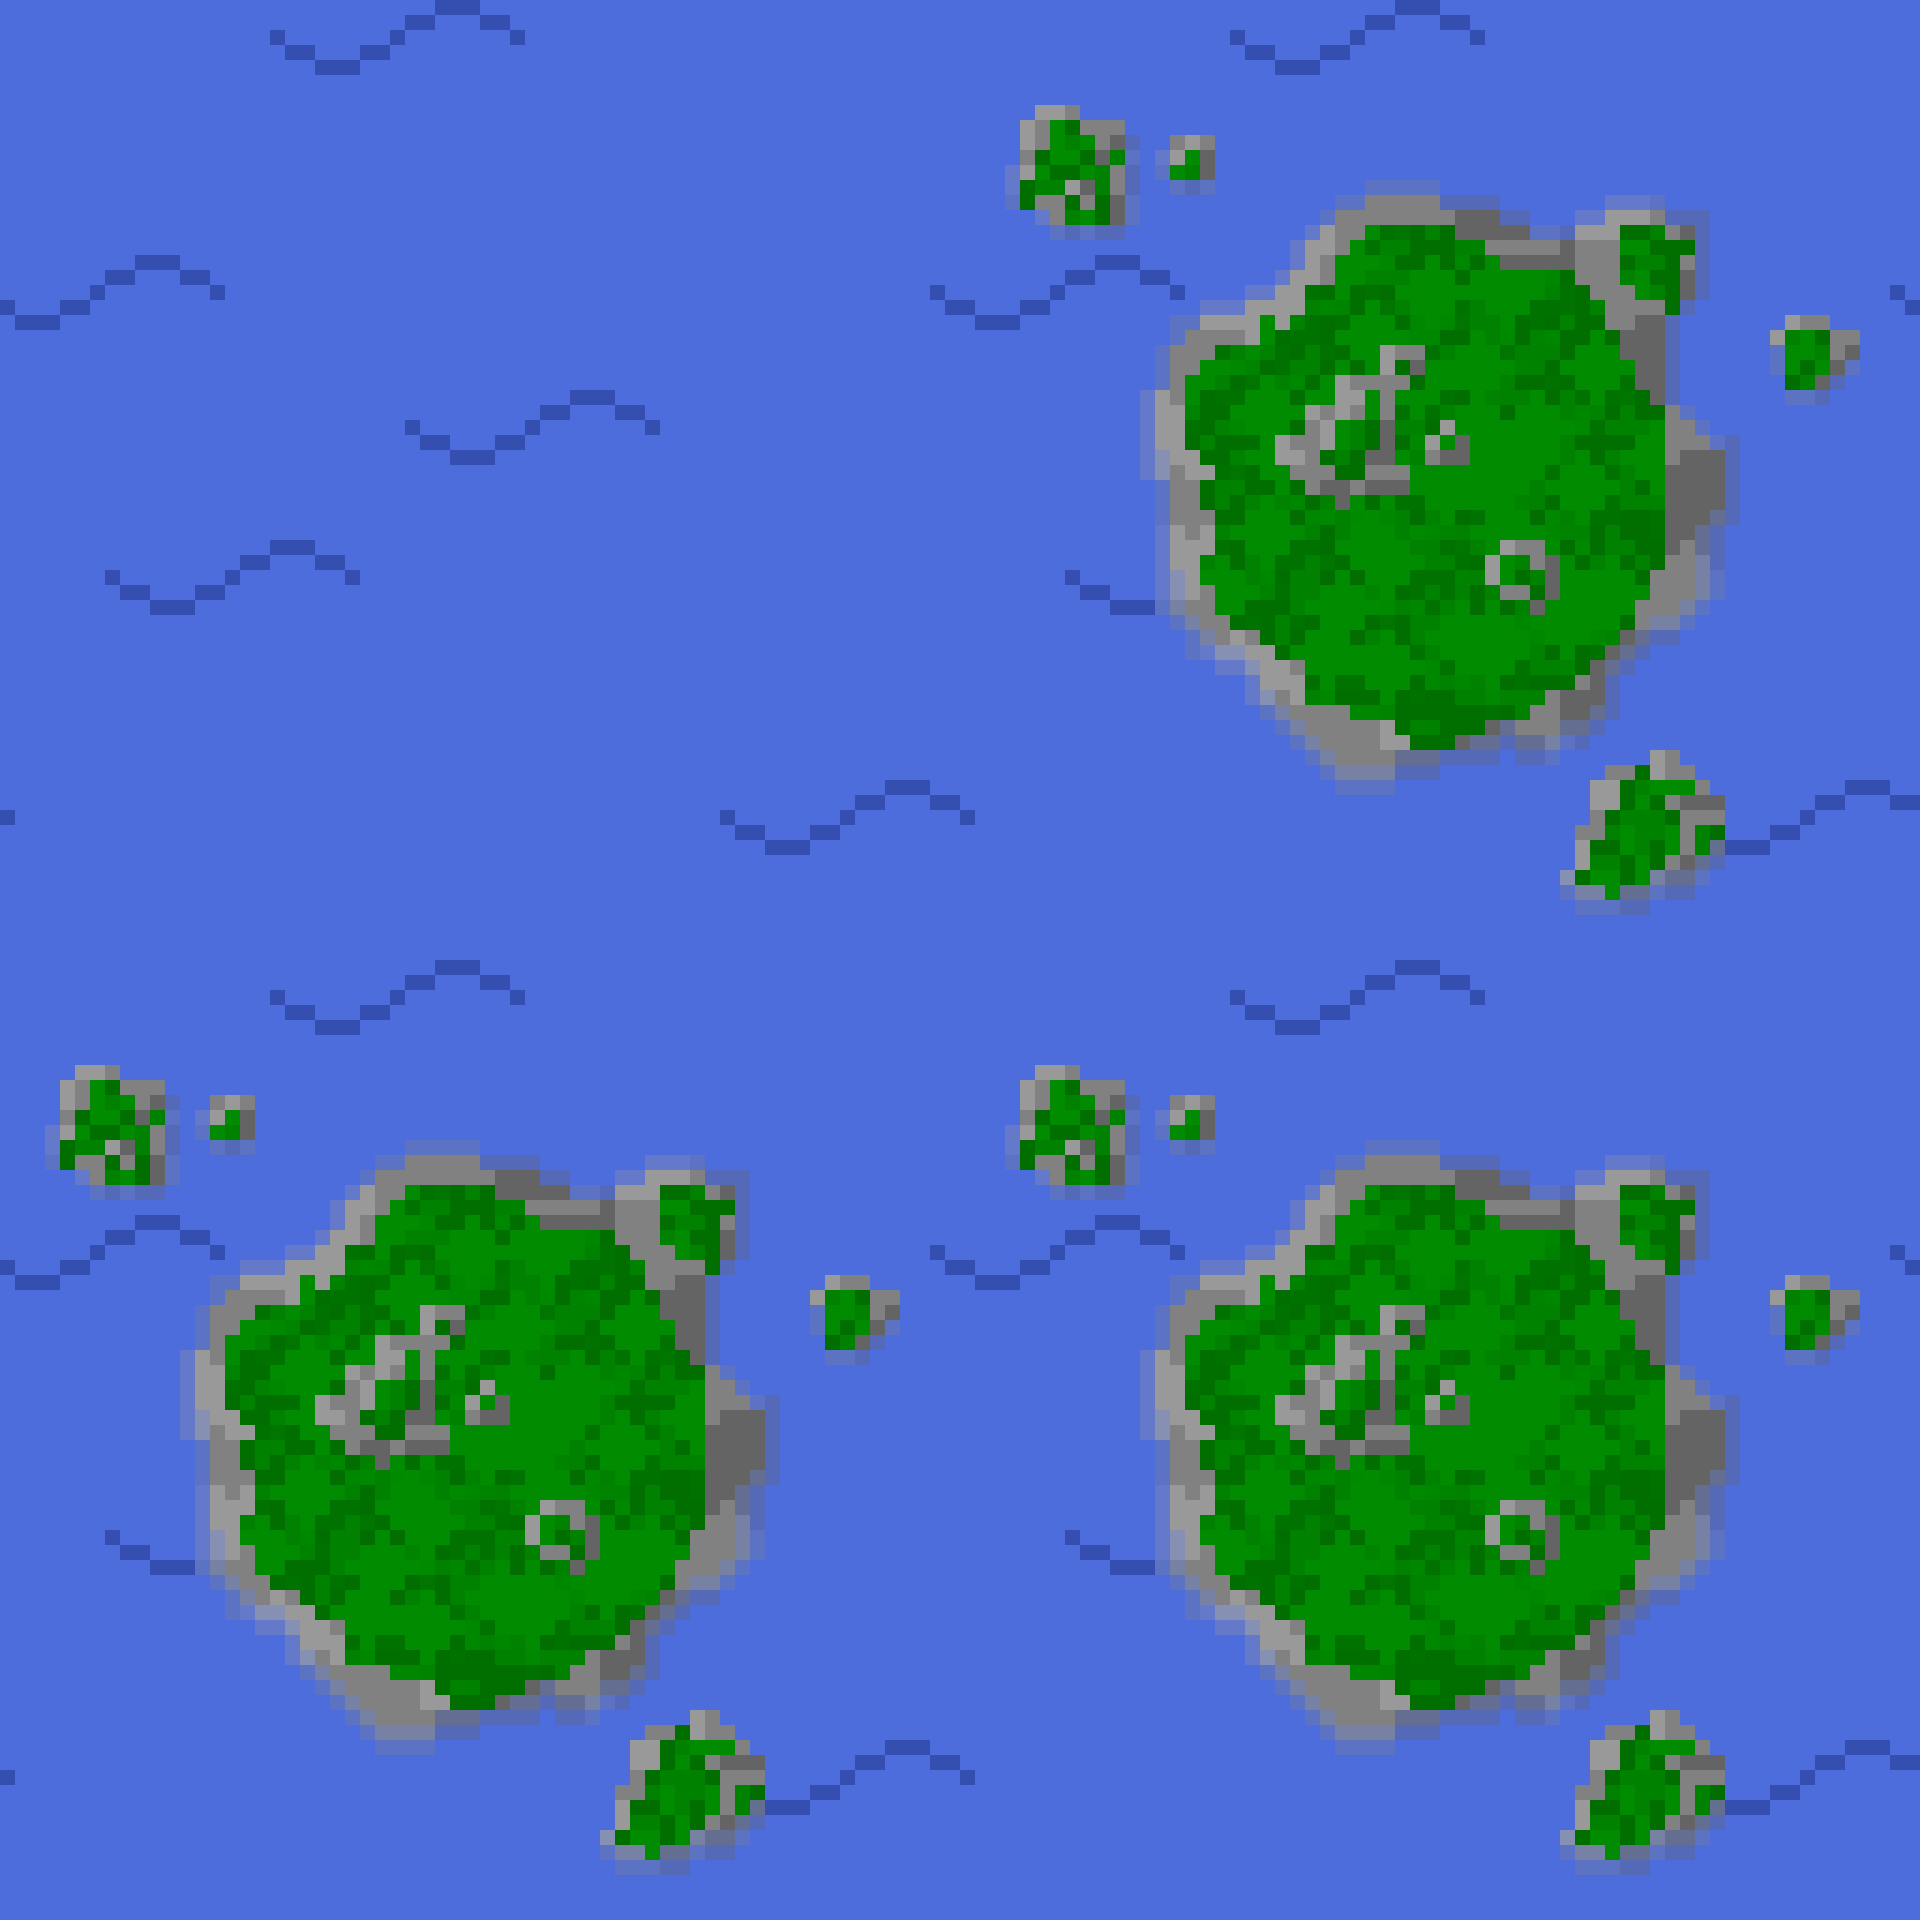
\includegraphics[width=0.8\textwidth]{img/sprites/2.png}
        \caption*{Case \texttt{NORD\_OUEST}}
    \end{minipage}
    \begin{minipage}{0.23\textwidth}
        \centering
        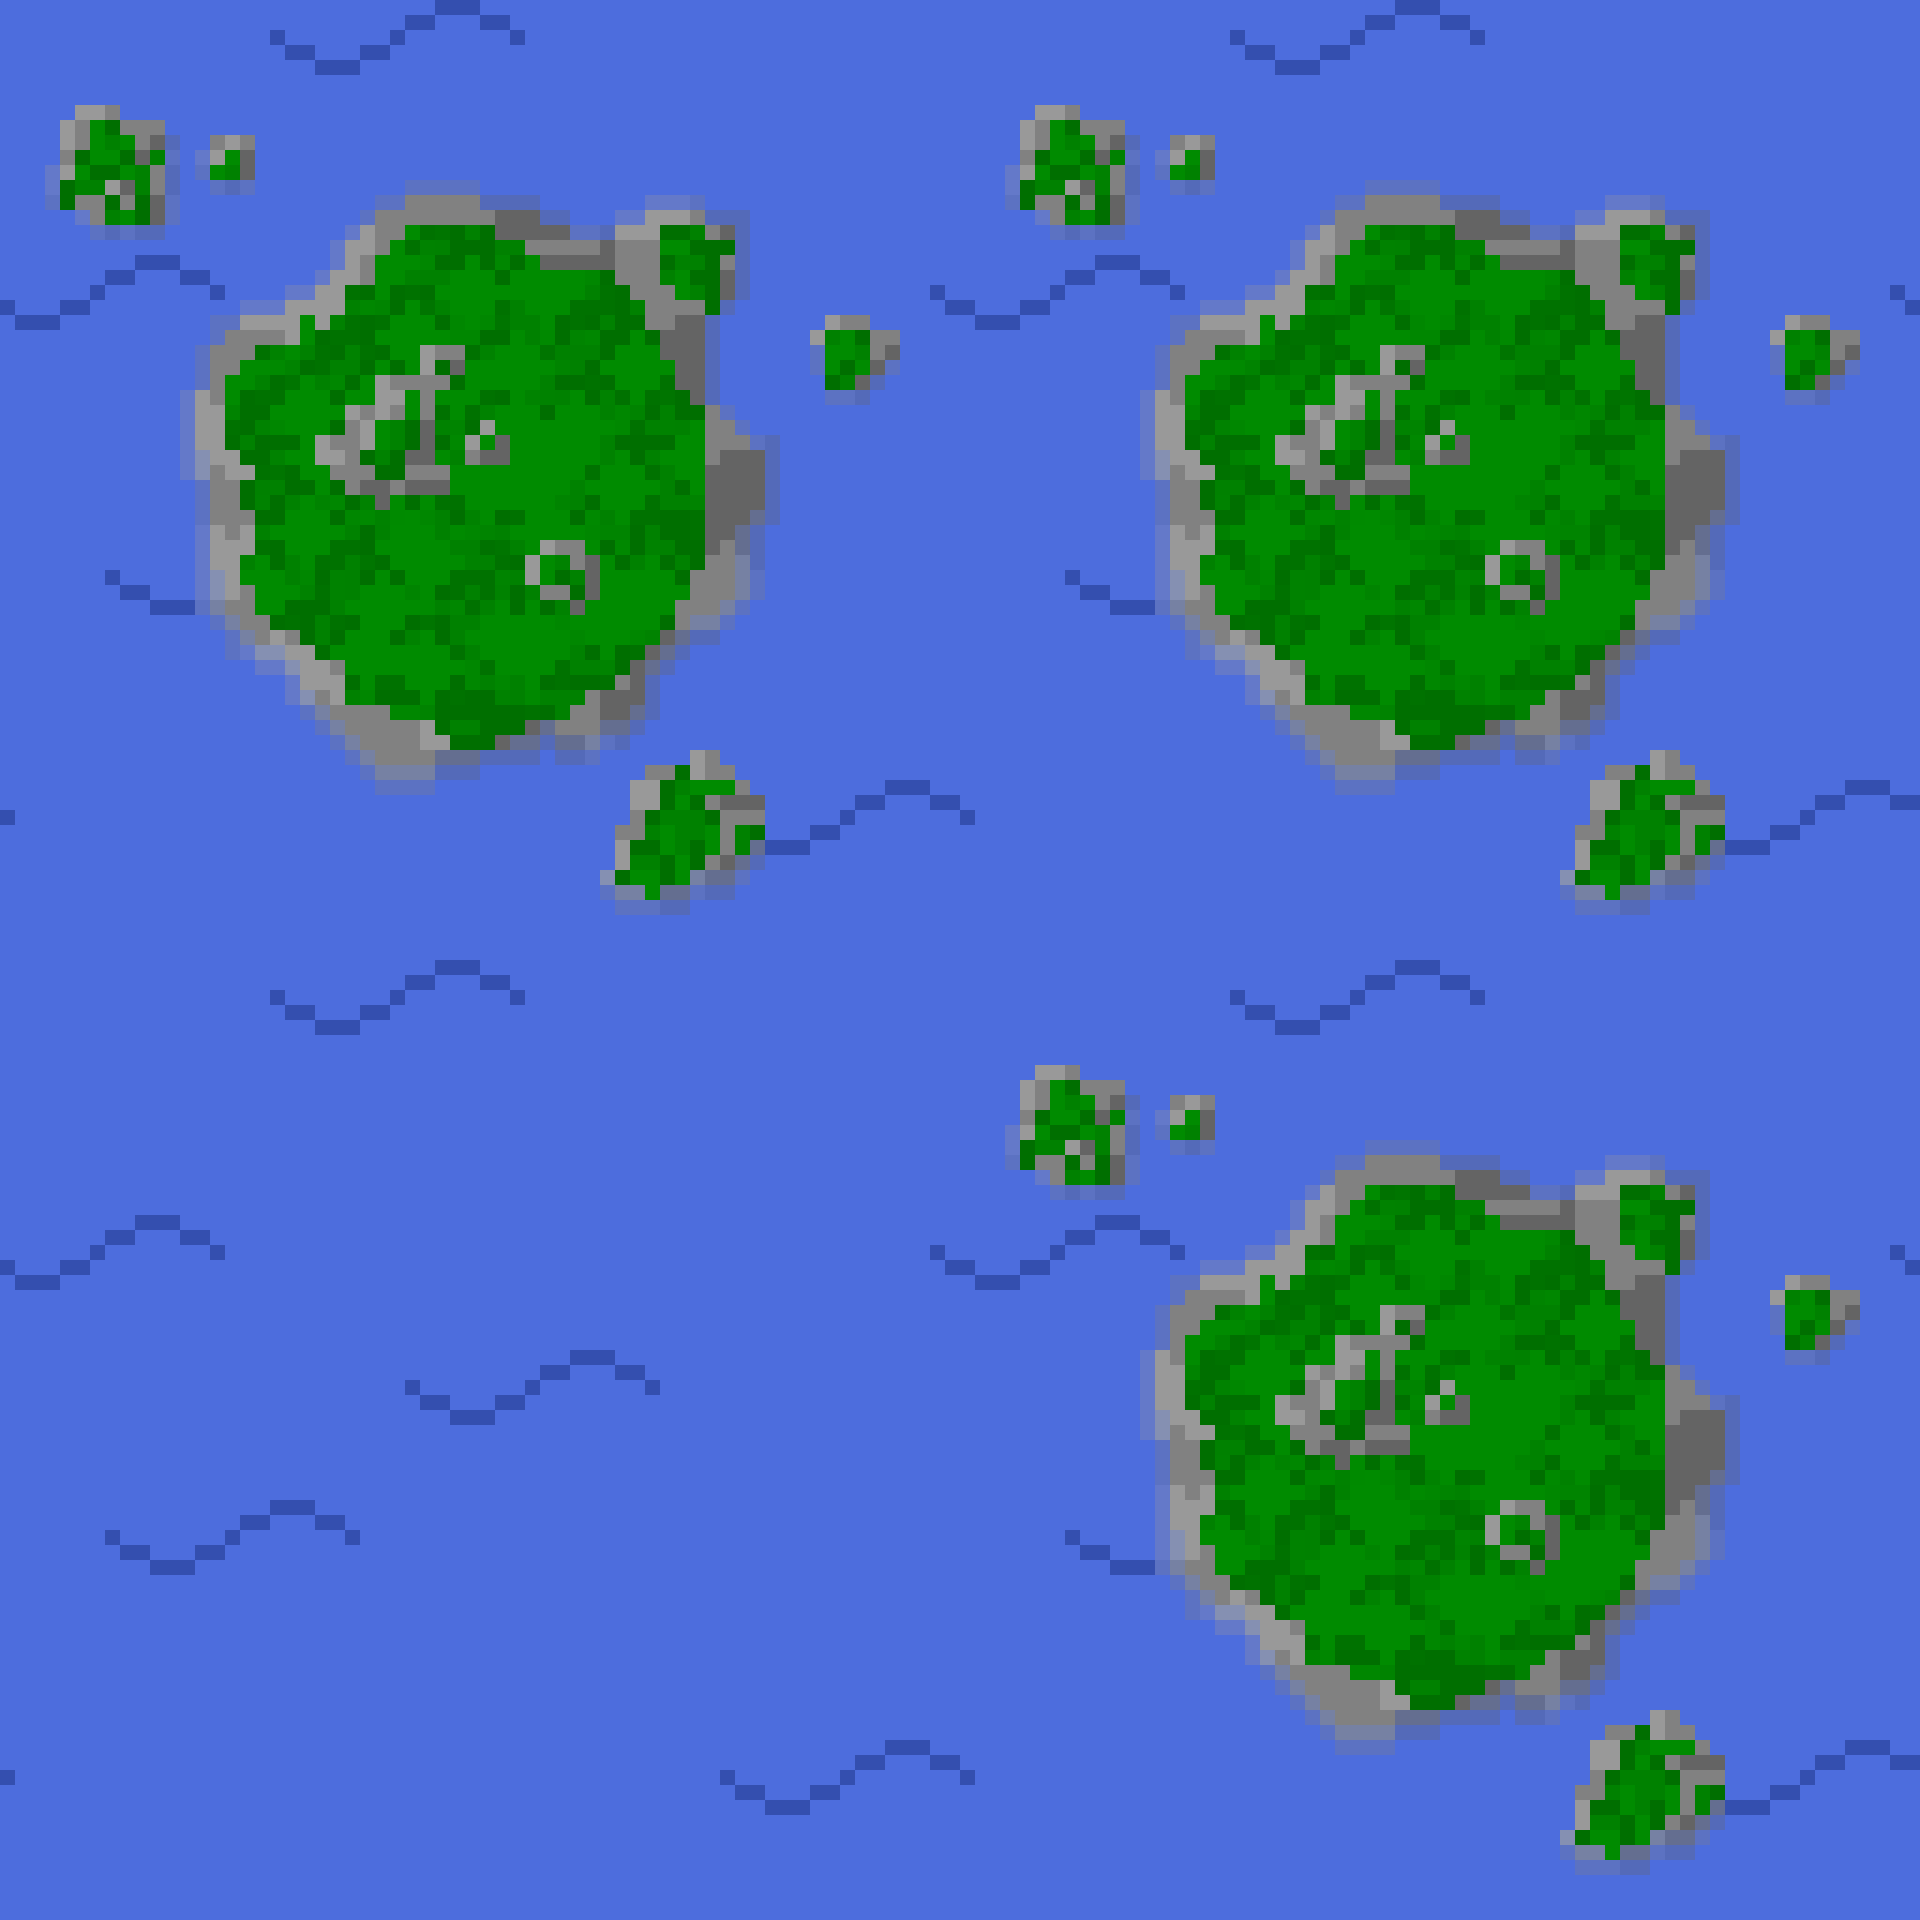
\includegraphics[width=0.8\textwidth]{img/sprites/3.png}
        \caption*{Case \texttt{SUD\_OUEST}}
    \end{minipage}
    \begin{minipage}{0.23\textwidth}
        \centering
        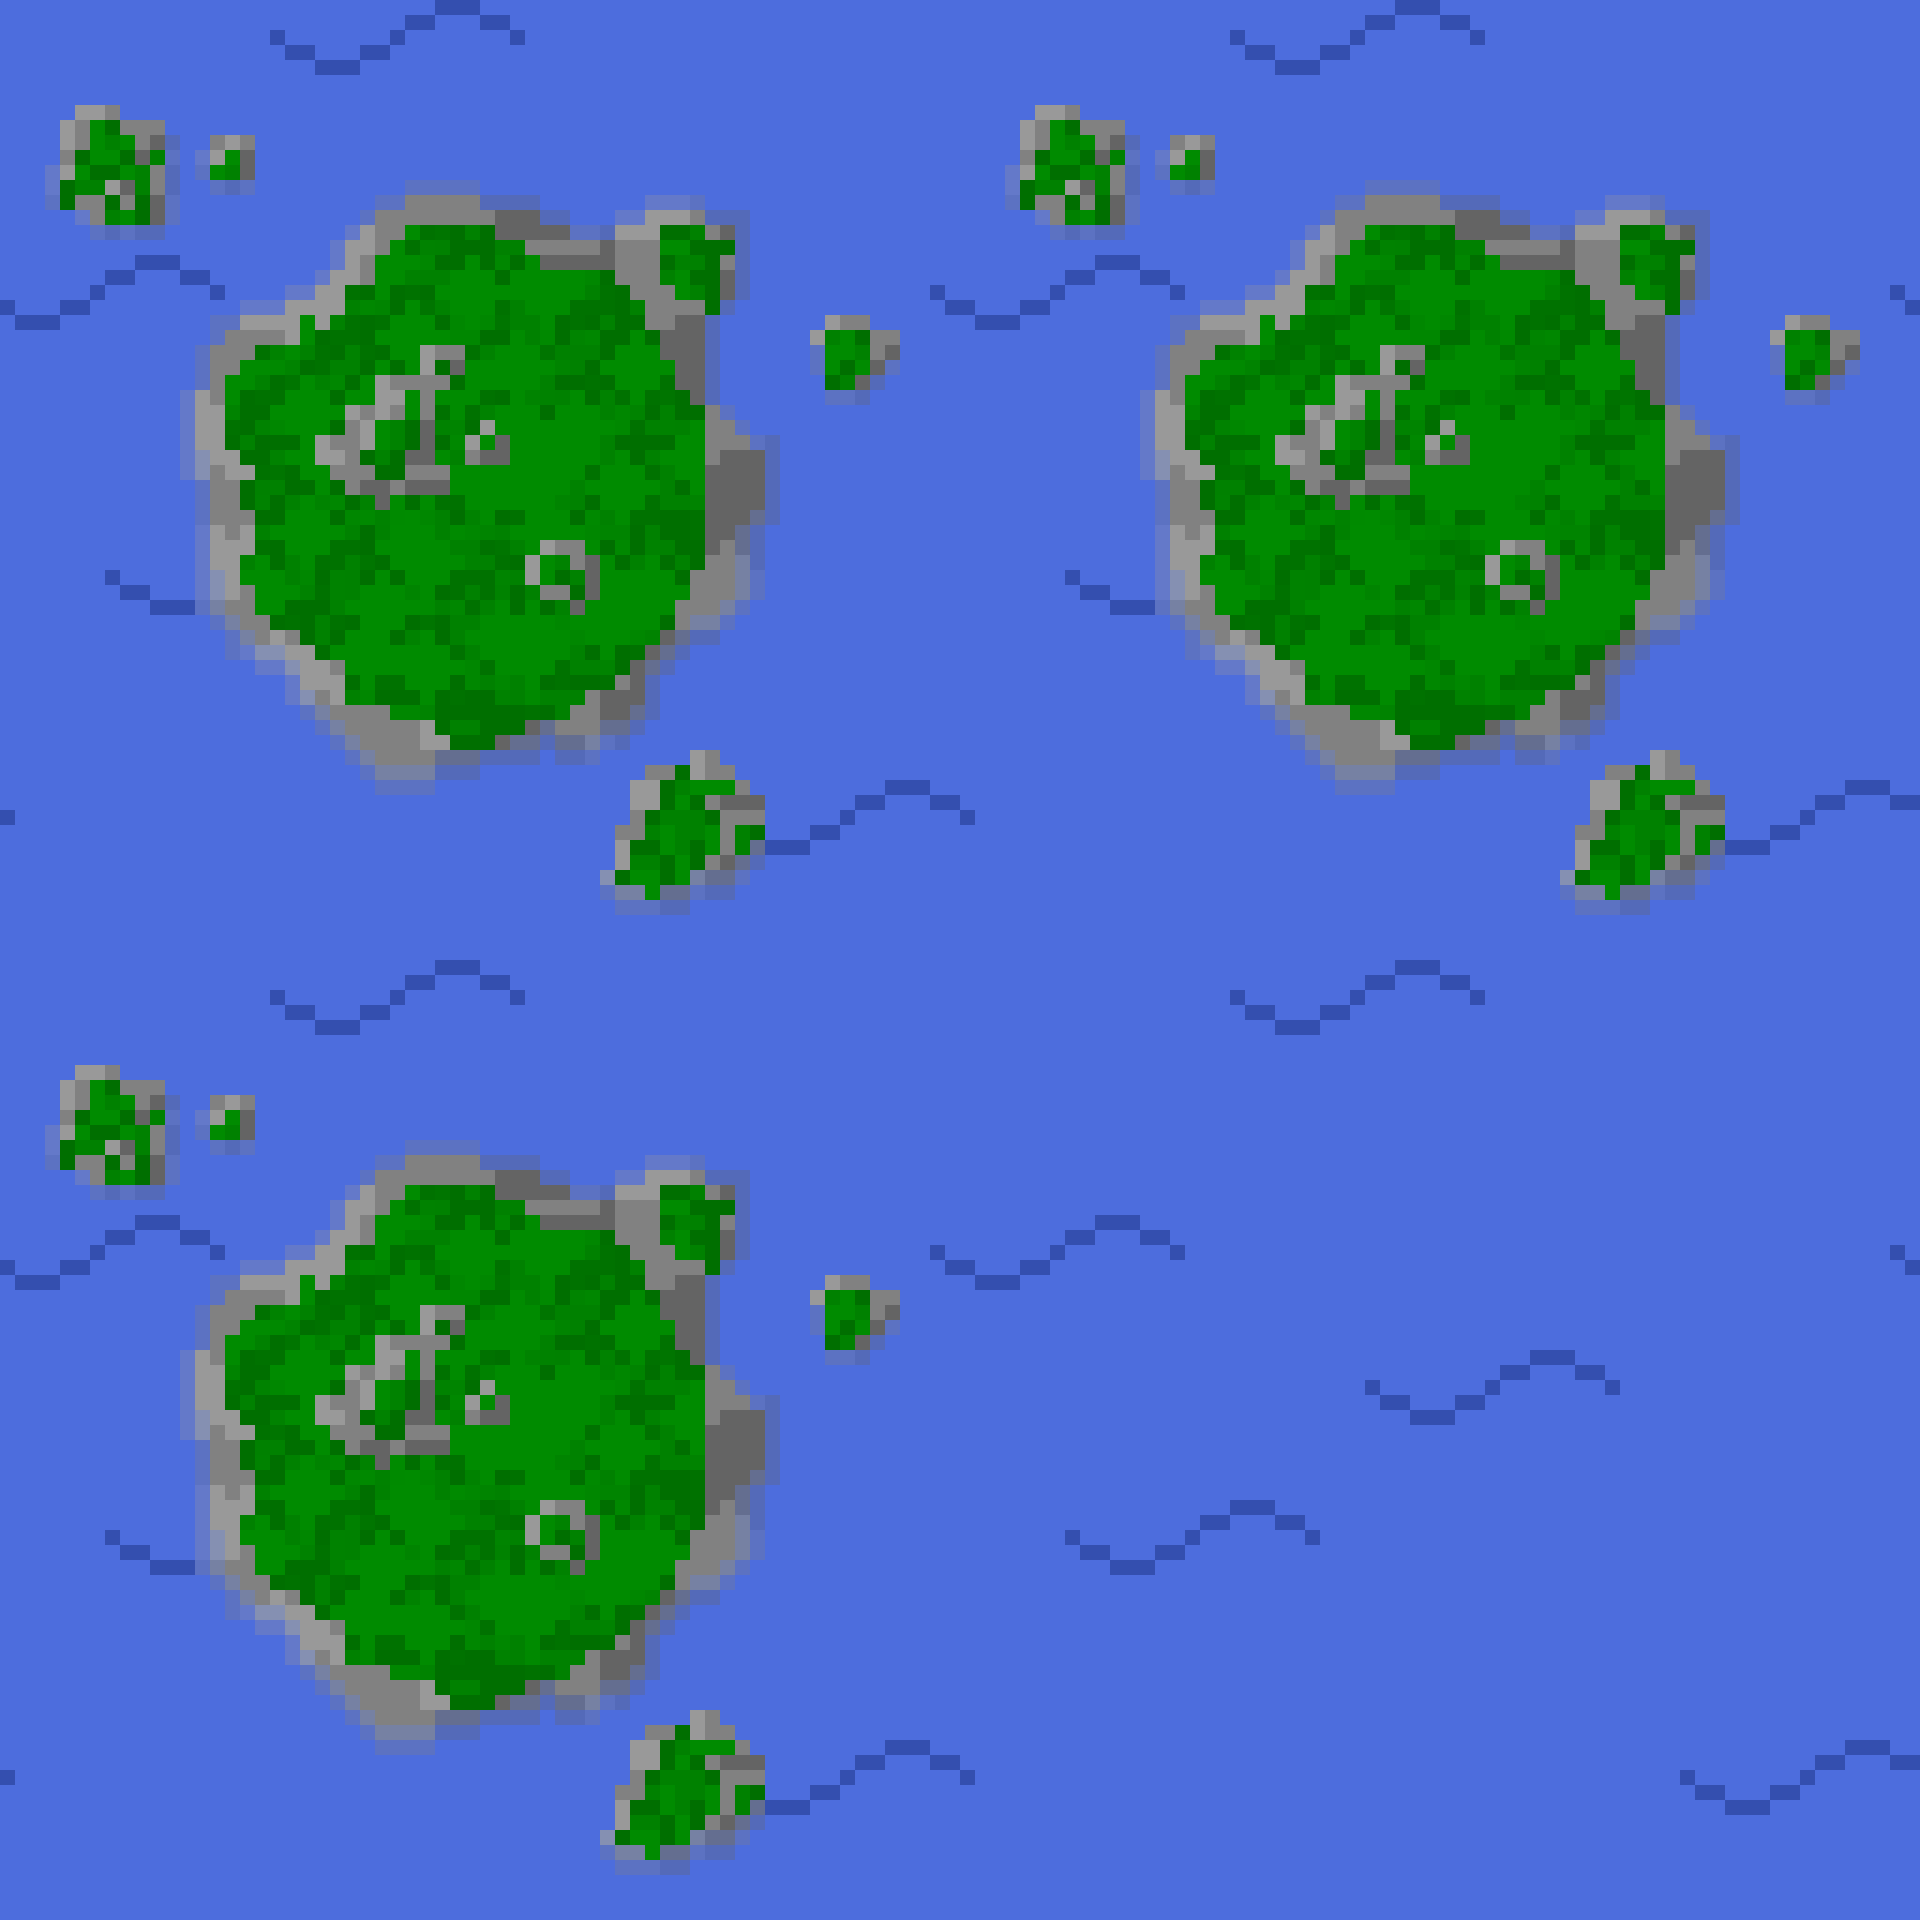
\includegraphics[width=0.8\textwidth]{img/sprites/4.png}
        \caption*{Case \texttt{SUD\_EST}}
    \end{minipage}
\end{figure}

\begin{figure}[h]
    \centering
    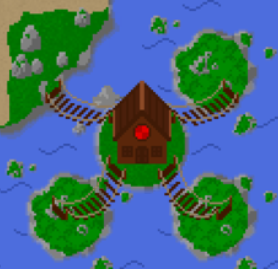
\includegraphics[width=0.2\textwidth]{img/case_village.png}
    \caption*{Un village}
\end{figure}

\newpage
Dans l'interface, le nord est toujours vers le haut de l'écran, l'est vers la
droite, et ainsi de suite.

Dans l'encodage d'une carte:
\begin{itemize}
    \item
        l'orientation \texttt{NORD\_EST} est encodé par un \texttt{1}
    \item
        l'orientation \texttt{NORD\_OUEST} est encodé par un \texttt{2}
    \item
        l'orientation \texttt{SUD\_OUEST} est encodé par un \texttt{3}
    \item
        l'orientation \texttt{SUD\_EST} est encodé par un \texttt{4}
    \item
        un village est encodé par un \texttt{X}
\end{itemize}

\subsection{Village}
Un village est une case spéciale dont les 4 coins sont des îlots.
Un village peut être possédé par un joueur ou être neutre
\footnote{Un village neutre n'est possédé par aucun joueur.}.
Les joueurs commencent la partie en ne possédant qu'un seul village
\footnote{Selon la configuration de la carte, il est possible de capturer
un village avant le début de la partie.}.

\subsection{Emplacements}
Un emplacement représente l'intersection de quatre cases adjacentes.
On dit que ces quatre cases \emph{bordent} l'emplacement.
Il y a donc $(\mathtt{largeur} - 1) \times (\mathtt{hauteur} - 1)$ emplacements.

Chaque emplacement peut être identifié par sa position, une paire
$(\mathtt{colonne}, \mathtt{ligne})$, où l'emplacement le plus au nord-ouest
possède la position $(0, 0)$, et l'emplacement le plus au sud-est possède
la position $(\mathtt{largeur} - 2, \mathtt{hauteur} - 2)$.
Les coordonnées d'un emplacement correspondent donc aux coordonnées de la case
directement au nord-ouest de cet emplacement.

\begin{figure}[h]
    \centering
    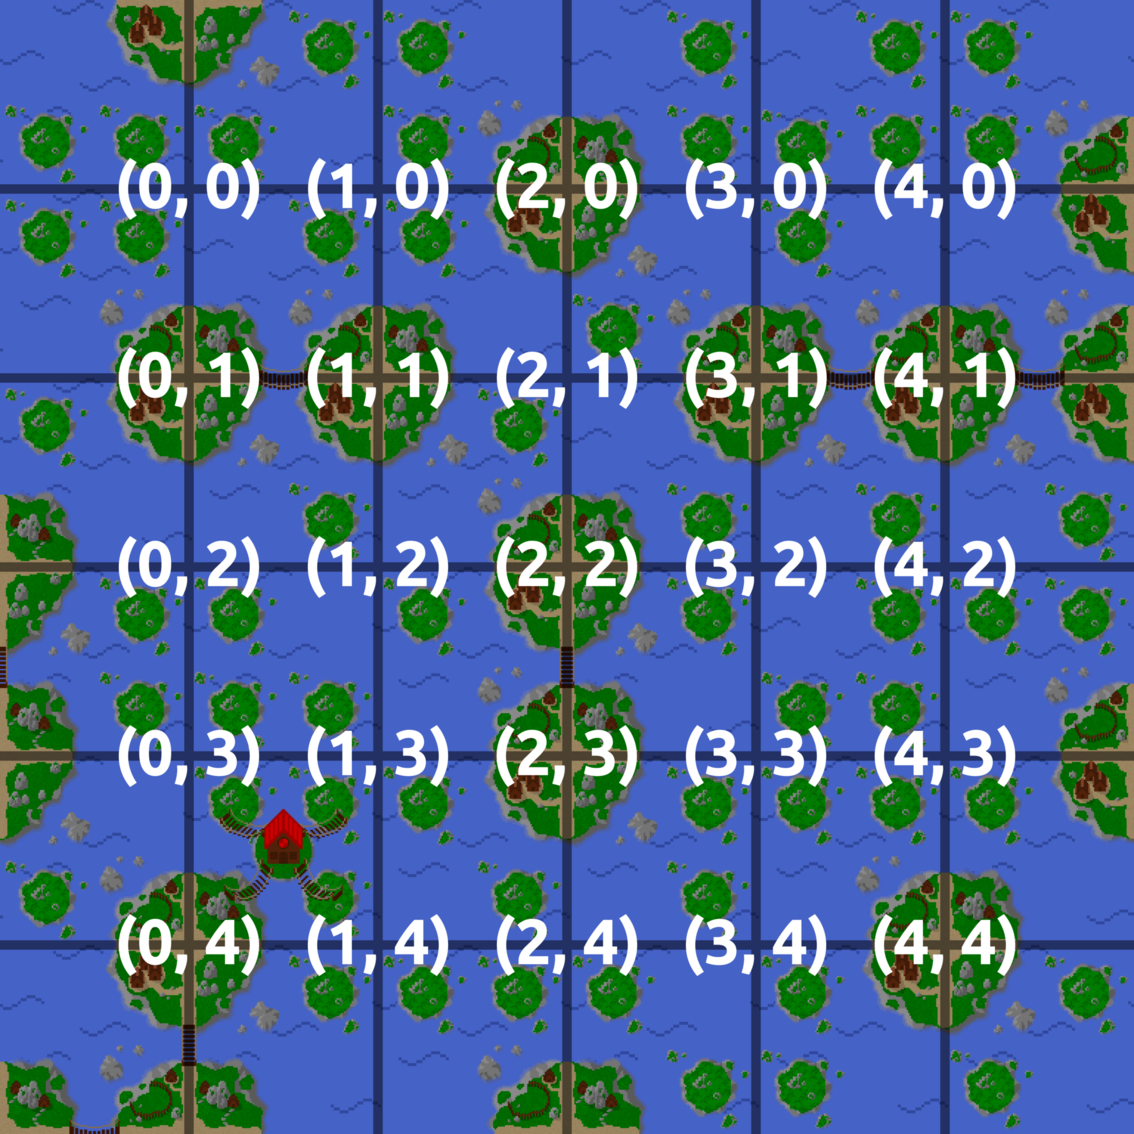
\includegraphics[width=0.4\textwidth]{img/sprites/emplacements.png}
    \caption{Coordonnées des emplacements de la carte}
\end{figure}

Notez qu'il n'y a pas d'emplacemement sur les bords de la carte.

Chaque emplacement se voit attribuer un gain potentiel, qui permet d'obtenir du
score.
Ce gain est un entier, pouvant être positif, négatif, ou nul.

Cet encadré vous est offert pour comptabiliser le nombre de fois où vous
avez confondu case et emplacement dans votre code:

\begin{center}
    \begin{tikzpicture}
        \draw (0, 0) rectangle (8, 2);
    \end{tikzpicture}
\end{center}

\subsection{Îles}
Lorsque quatre îlots bordent un emplacement, une île se forme à cet
emplacement.
L'île persiste tant que quatre îlots bordent l'emplacement.
L'île disparait dès qu'une des quatre cases bordant l'emplacement ne fournit
plus d'îlot pour l'emplacement.

\begin{figure}[h]
    \centering
    \begin{minipage}{.35\textwidth}
        \centering
        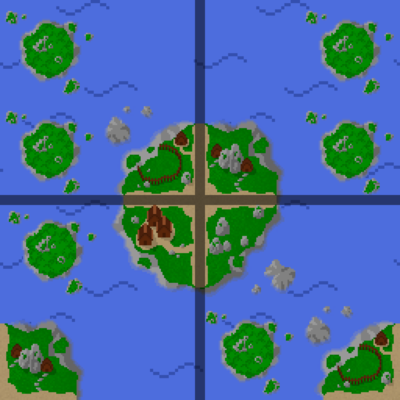
\includegraphics[width=0.75\textwidth]{img/sprites/ile.png}
        \caption{Île formée par quatre îlots}
    \end{minipage}
    \begin{minipage}{.6\textwidth}
        \centering
        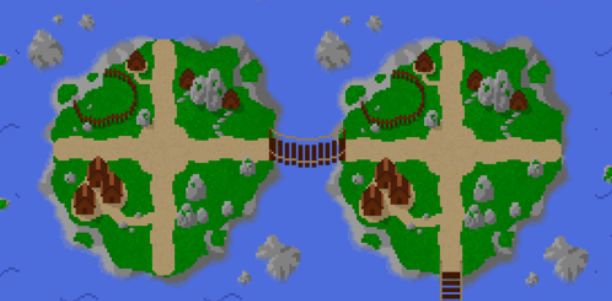
\includegraphics[width=0.9\textwidth]{img/pont.png}
        \caption{Deux îles connectées}
    \end{minipage}
\end{figure}

Deux îles sont connectées si elles sont adjacentes, c'est-à-dire, si elles
se situent sur deux emplacements côte-à-côte sur la même ligne ou la même
colonne.
Deux îles en diagonale ne sont pas considérées comme directement connectées.

\subsection{Rotation}\label{sec:rotation}
Les joueurs peuvent tourner à un certain coût les cases d'un quart de tour dans
le sens trigonométrique (anti-horaire).

\begin{figure}[h]
    \centering
    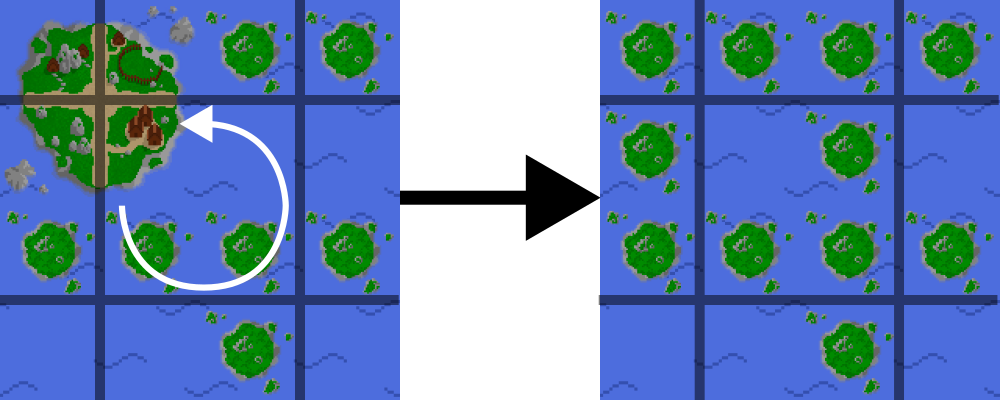
\includegraphics[width=0.7\textwidth]{img/sprites/rotation.png}
    \caption{Rotation d'une case}
\end{figure}

Il est impossible pour un joueur de faire tourner un village, ou de faire
tourner une case gelée.

\section{Territoire}
Le territoire d'un joueur représente le réseau des îles connectées,
reliées à au moins un village contrôlé par le joueur.

\begin{figure}[h]
    \centering
    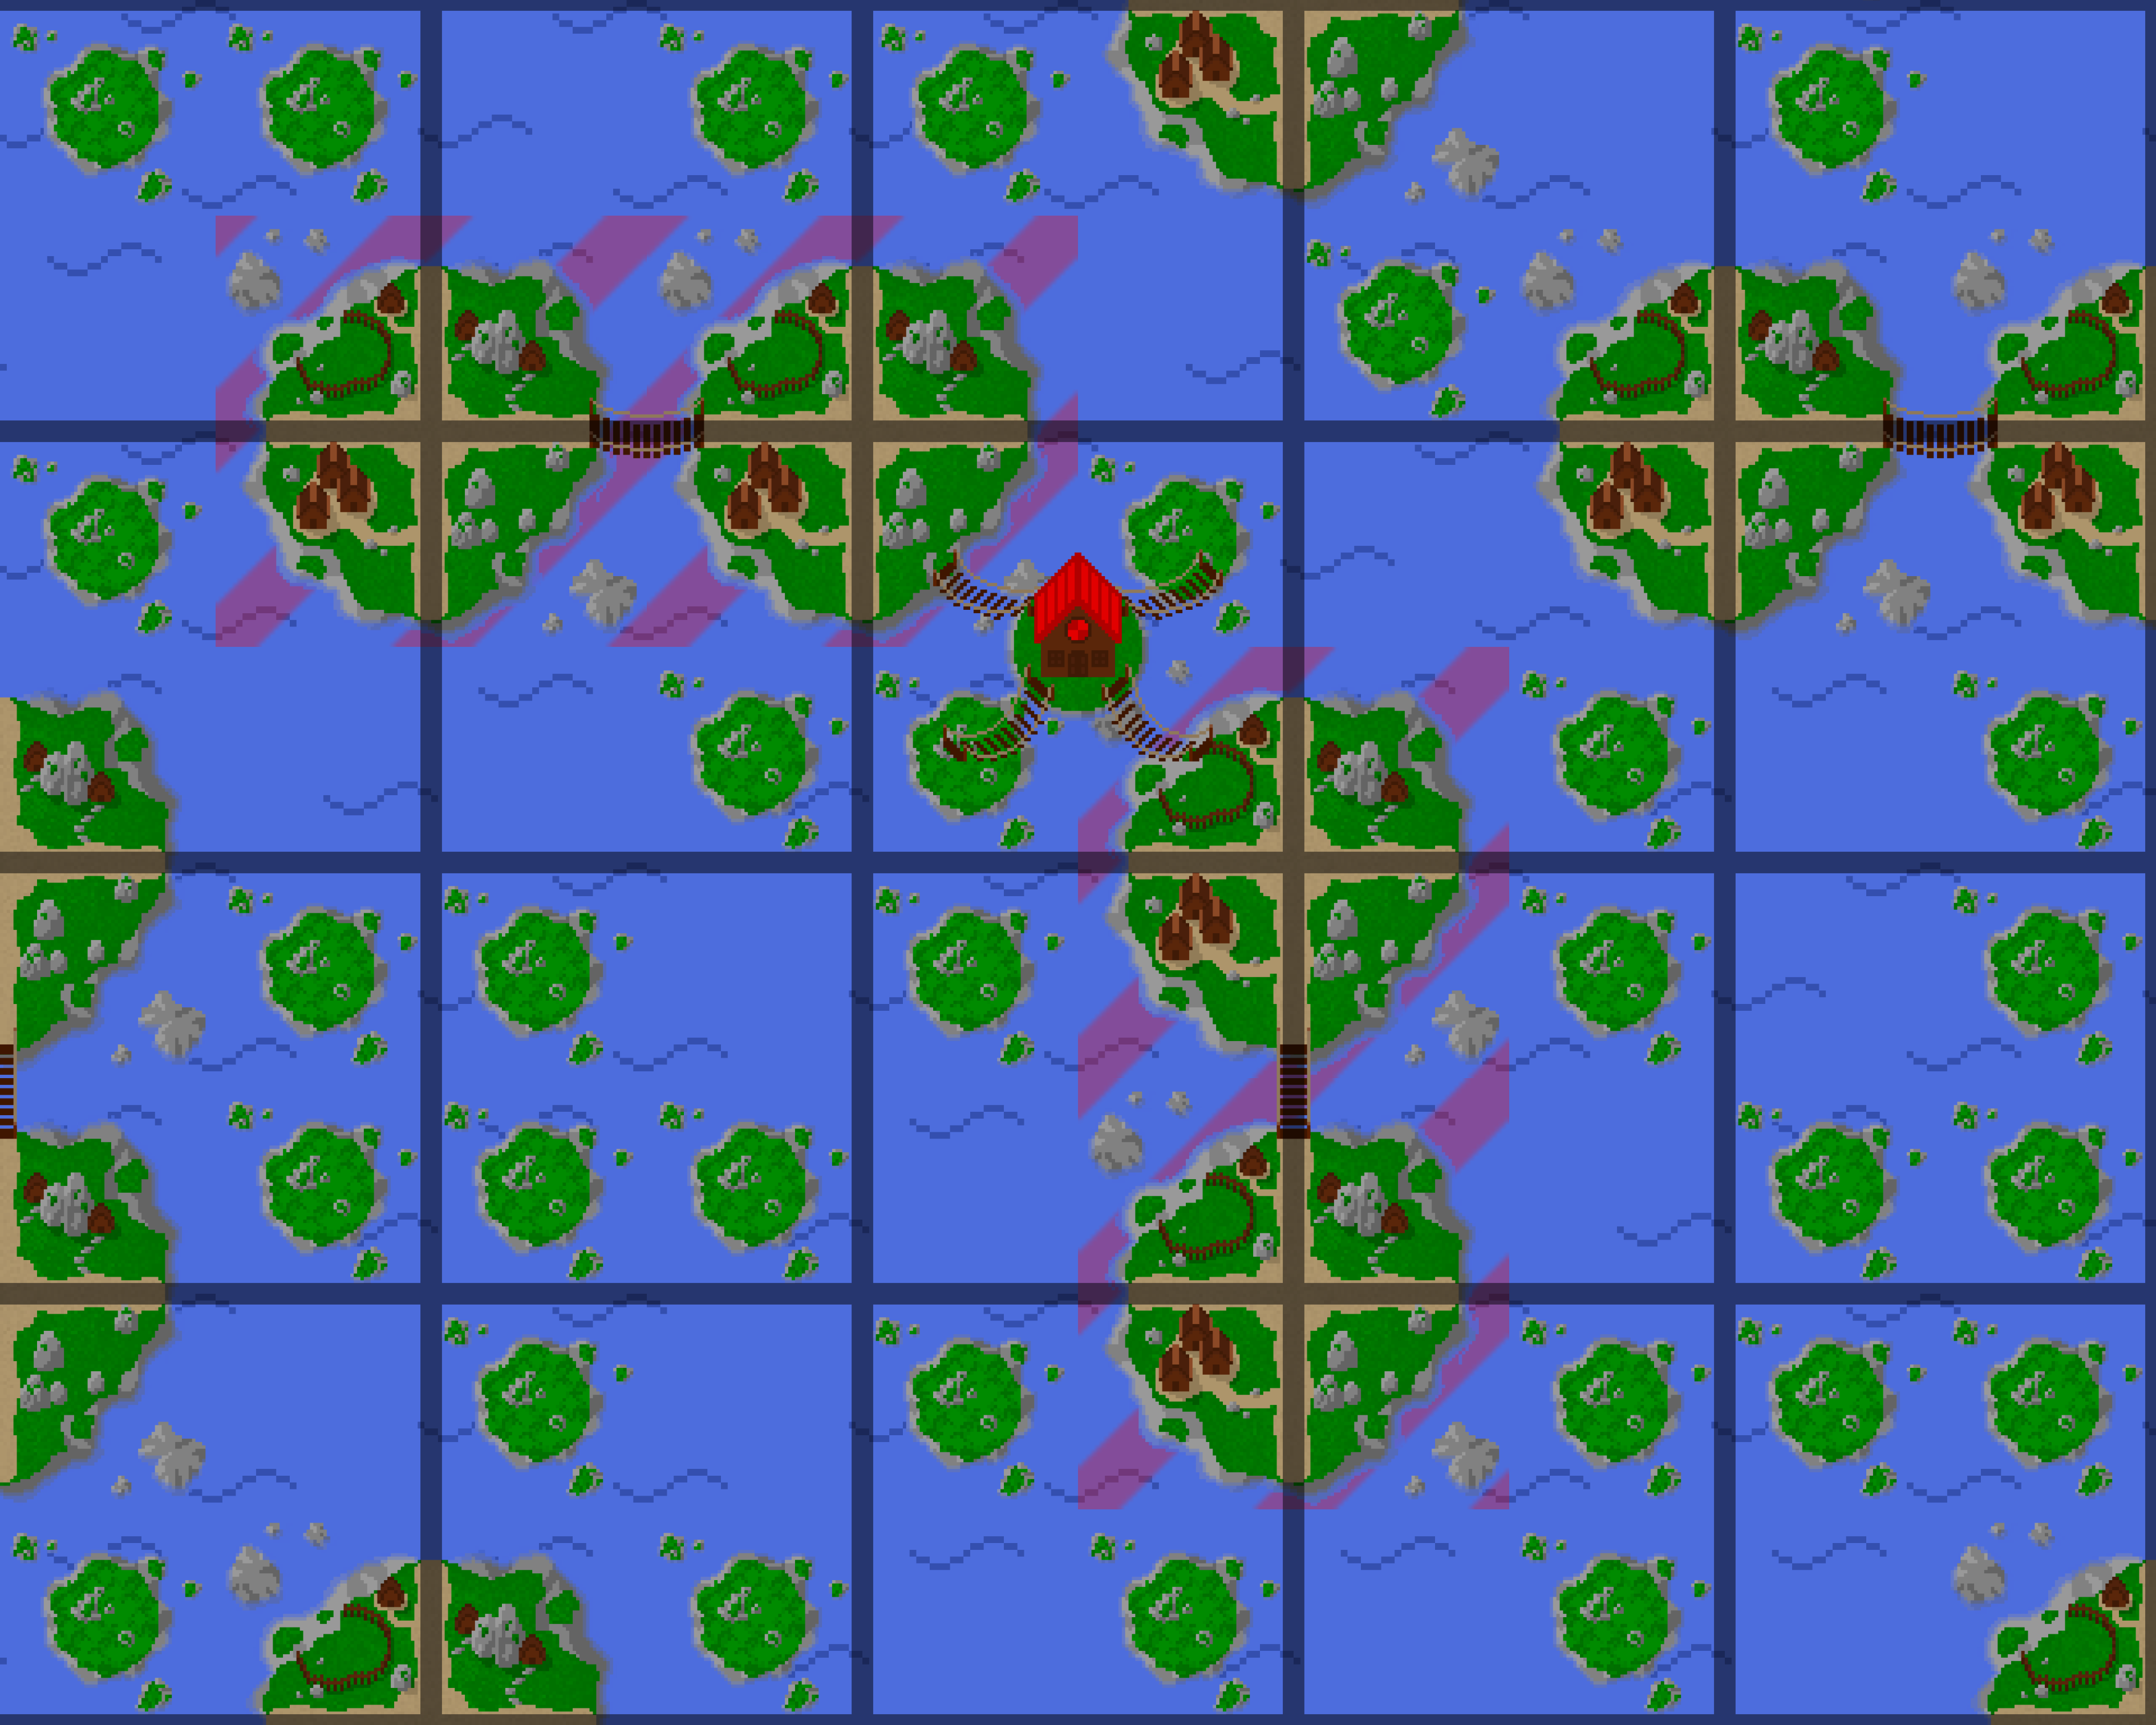
\includegraphics[width=0.4\textwidth]{img/sprites/territoire.png}
    \caption{Un territoire de quatre îles}
\end{figure}

Si une chaîne d'îles relie un village de chaque joueur, alors ces îles
appartiennent au territoire des deux joueurs.

Si, à la fin d'un tour, un village neutre appartient au territoire d'un unique
joueur, alors le joueur capture le village de manière définitive.
Si un village neutre appartient au territoire des deux joueurs, il reste neutre.

Le territoire n'est pas forcément connexe.
Si vous disposez de plusieurs villages, chaque village peut posséder son
propre réseau d'îles qui contribuera à votre territoire.

\newpage
\section{Points d'action}
Chaque tour, un joueur commence avec \texttt{TOUR\_POINTS\_ACTION} points
d'action.
Les points d'action ne servent qu'à tourner des cases.

La rotation d'une case qui borde au moins un emplacement du territoire adverse
demande \texttt{COUT\_ROTATION\_ENNEMI} points d'action.
Sinon, la rotation demande \texttt{COUT\_ROTATION\_STANDARD} point d'action.

Toutes les autres actions ne consomment aucun point d'action, et peuvent
être répétées sans contraintes.

\section{Aigles}
Un aigle est une créature divine qui peut être présent sur un emplacement
dès le début de la partie, sous la forme d'un œuf.

Au début de la partie, plusieurs œufs peuvent être disposés sur la carte.
Chaque œuf possède un certain tour d'éclosion, avant lequel l'aigle n'est
pas capturable. 
Une fois son tour d'éclosion atteint, un aigle sauvage sort de l'œuf
et reste sur son emplacement jusqu'à sa capture.

À la fin d'un tour, si l'emplacement d'un aigle sauvage appartient au
territoire d'un unique joueur, le joueur capture l'aigle.
Si l'emplacement d'un aigle sauvage appartient au territoire des deux joueurs,
l'aigle reste sauvage.
Plusieurs aigles et œufs peuvent se trouver sur un même emplacement.

Un aigle capturé peut être déplacé autant fois que souhaité lors d'un même tour
et n'importe où sur la carte.
Plusieurs aigles peuvent se situer sur le même emplacement, indépendamment
de s'ils sont sauvage ou non, de leur propriétaire, ni de leur effet.

% TODO: images œufs/aigles

\subsection{Pouvoirs}

Les aigles sont tous dotés d'un pouvoir et d'une puissance.
La puissance est un entier dont la signification est spécifique au pouvoir.
On détaillera ce que représente cette donnée plus tard dans le sujet.

Il existe deux types d'aigles~: les aigles éphémères et les aigles persistants.
Les aigles éphémères ont un pouvoir qui ne s'active qu'une fois avant de
disparaître à jamais.
Les aigles persistants ont un pouvoir qui perdure tant qu'ils restent sur la
carte.

\paragraph{Rayon d'action}
Certains aigles ont un pouvoir dont l'effet s'applique sur des cases ou des
emplacements autour de l'aigle.
La portée de l'effet formera alors un carré, dont la taille dépend de la
puissance de l'aigle.

Par exemple, si l'effet d'un aigle s'applique sur des emplacements,
une puissance de 0 appliquera l'effet uniquement sur l'emplacement où se
situe l'aigle.
Une puissance de 1 appliquera l'effet sur les neuf emplacements autour de
l'aigle.

\begin{figure}[h]
    \centering
    \begin{minipage}{.4\textwidth}
        \centering
        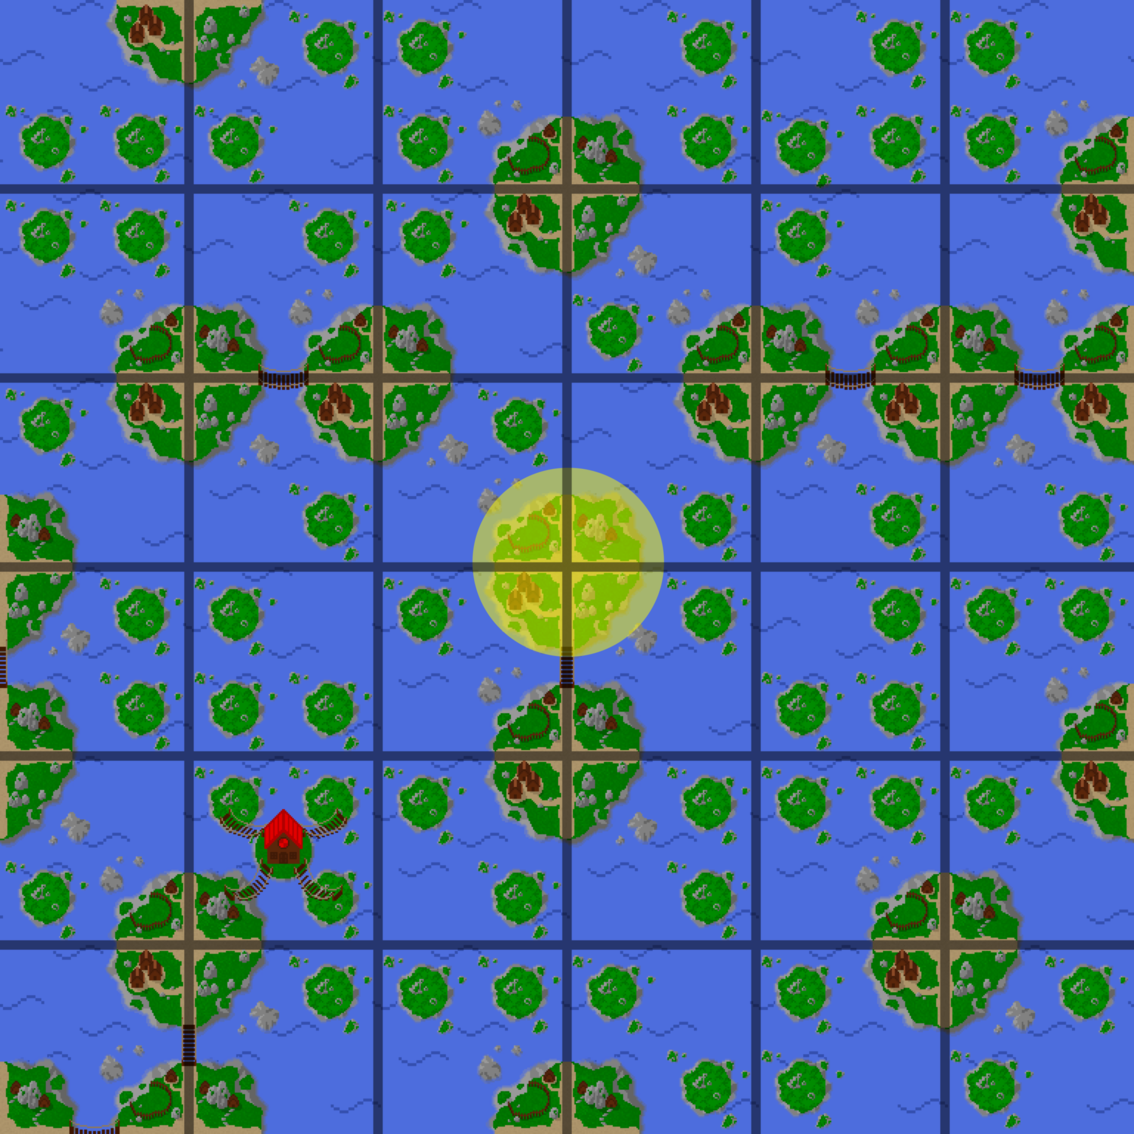
\includegraphics[width=.7\textwidth]{img/sprites/emplacement0.png}
        \caption*{La portée d'un aigle de puissance 0}
    \end{minipage}
    \begin{minipage}{.4\textwidth}
        \centering
        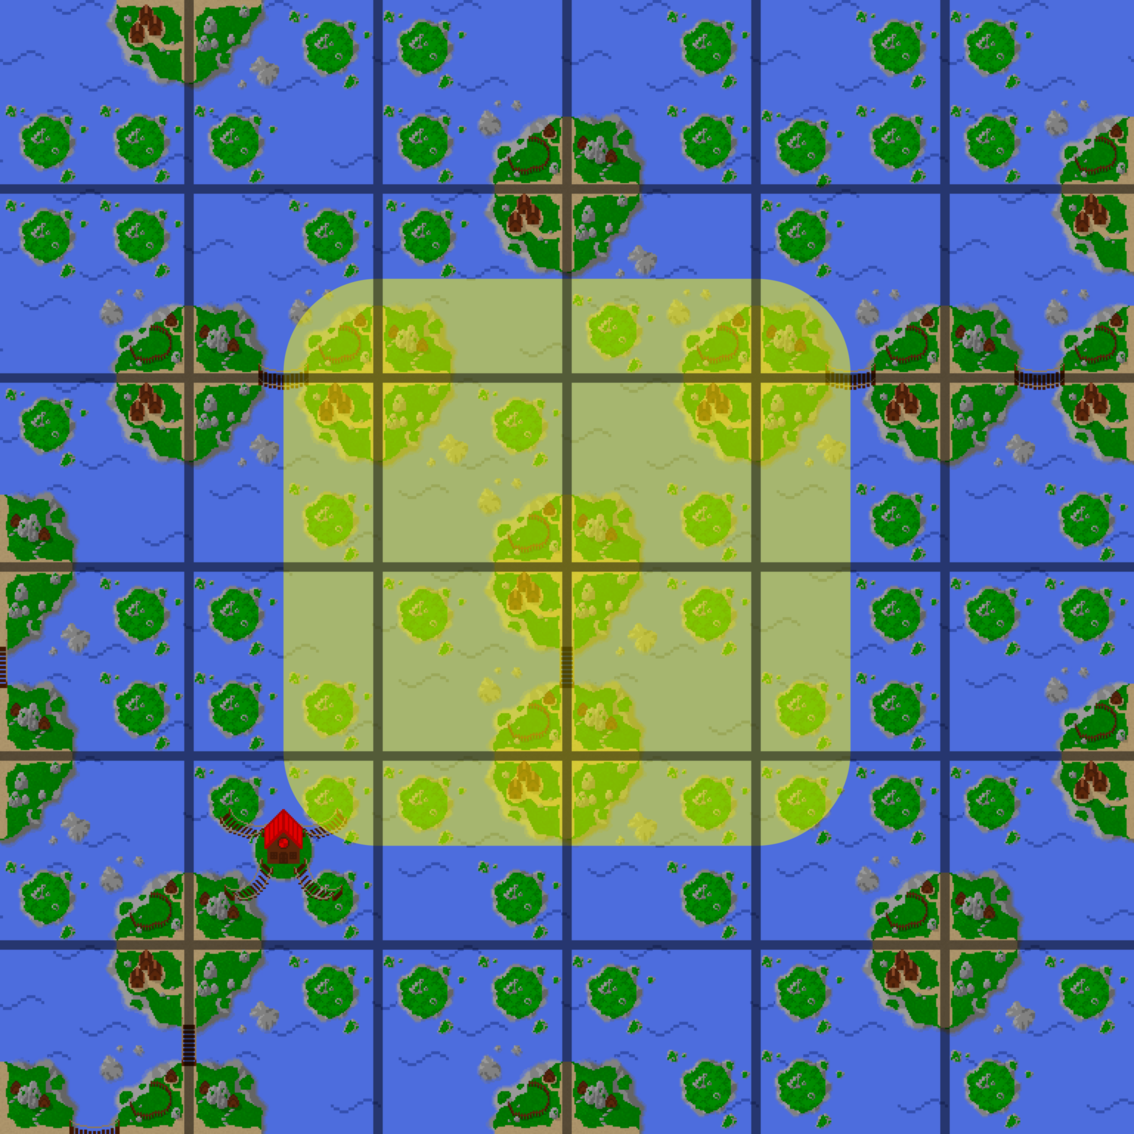
\includegraphics[width=.7\textwidth]{img/sprites/emplacement1.png}
        \caption*{La portée d'un aigle de puissance 1}
    \end{minipage}
\end{figure}

Si l'effet d'un aigle s'applique sur des cases, alors l'effet s'applique sur
toutes les cases bordant les emplacements impliqués.
Une puissance de 0 appliquera donc l'effet sur les 4 cases bordant l'emplacement
de l'aigle.

\begin{figure}[h]
    \centering
    \begin{minipage}{.4\textwidth}
        \centering
        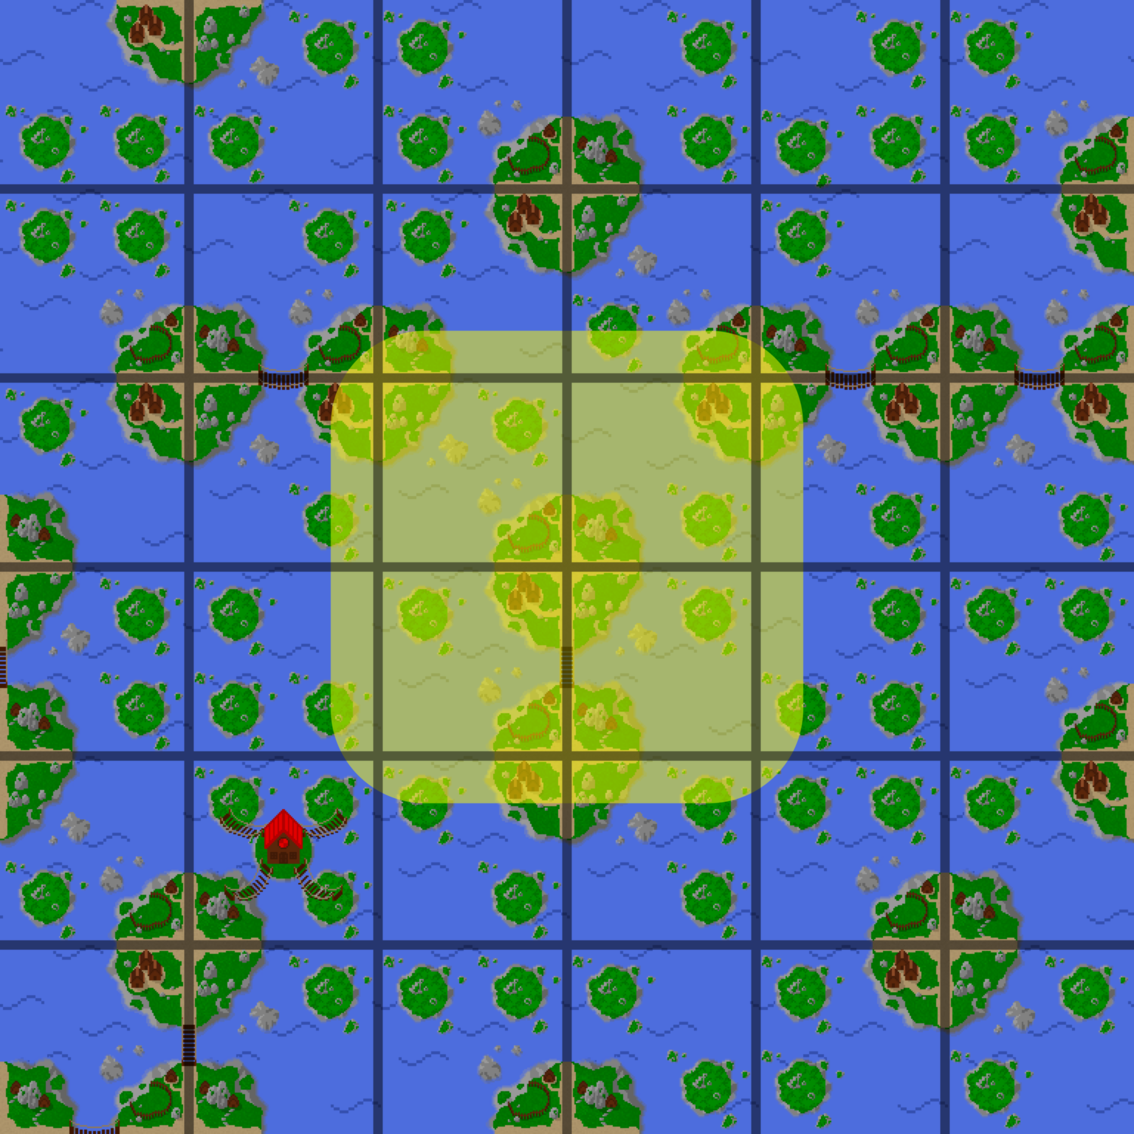
\includegraphics[width=.7\textwidth]{img/sprites/case0.png}
        \caption*{Cases affectées par un aigle de puissance 0}
    \end{minipage}
    \begin{minipage}{.4\textwidth}
        \centering
        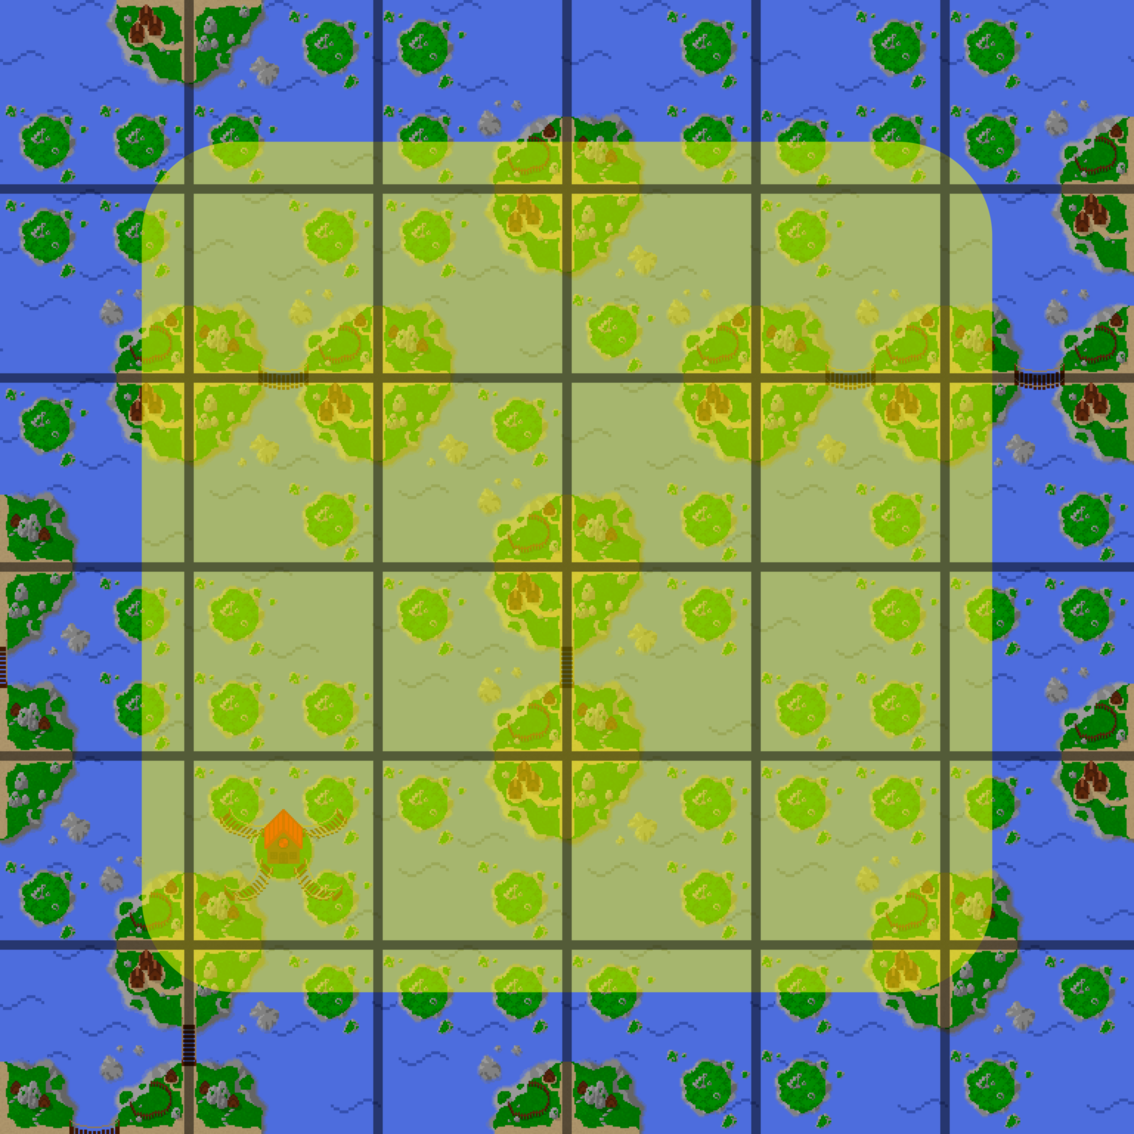
\includegraphics[width=.7\textwidth]{img/sprites/case1.png}
        \caption*{Cases affectées par un aigle de puissance 1}
    \end{minipage}
\end{figure}

\newpage

\begin{minipage}{.75\textwidth}
    \paragraph{Aigle de vie}
    L'aigle de vie est un aigle éphémère qui, une fois activé, attribue au joueur
    sa puissance en points d'actions pour le tour actuel.
    
    La puissance d'un aigle de vie peut avoir n'importe quelle valeur, positive
    ou négative.
\end{minipage}
\begin{minipage}{.2\textwidth}
    \centering
    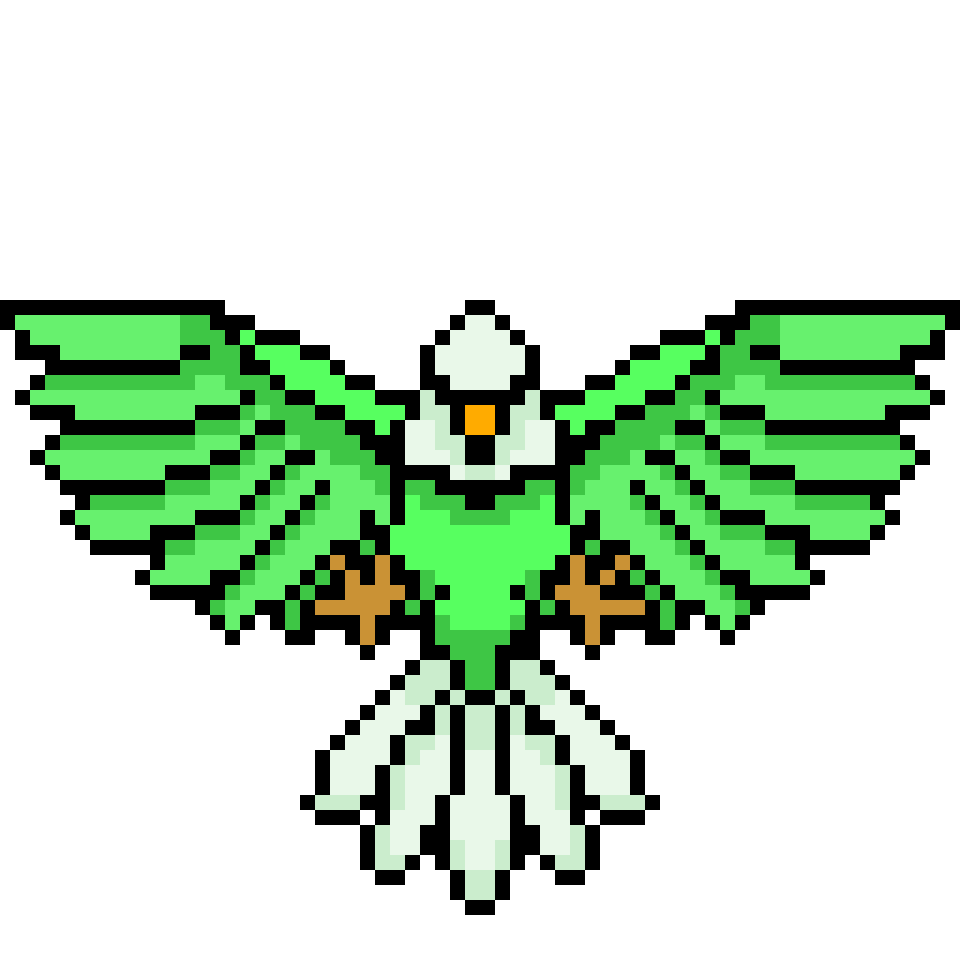
\includegraphics[width=.8\textwidth]{img/sprites/aigle_vie.png}
\end{minipage}

\begin{minipage}{.75\textwidth}
    \paragraph{Aigle météore}
    L'aigle météore est un aigle éphémère qui, une fois activé, tourne deux fois
    toutes les cases non gelées dans son rayon d'action.
    Sa puissance est une portée, et ne peut donc pas être négative.
\end{minipage}
\begin{minipage}{.2\textwidth}
    \centering
    
\includegraphics[width=.8\textwidth]{img/sprites/aigle_meteore.png}
\end{minipage}

\begin{minipage}{.75\textwidth}
    \paragraph{Aigle de feu}
    L'aigle de feu est un aigle persistant qui multiplie le gain de l'emplacement
    sur lequel il se trouve.
    Sa puissance indique le multiplicateur qui s'applique sur le gain de
    l'emplacement.
    Ce multiplicateur peut être négatif.

    L'effet des aigles de feu est cumulable de manière multiplicative.
    Par exemple, s'il y a deux aigles de feu de puissance $2$ et $-5$ sur un même
    emplacement, alors le gain de l'île est multiplié par $-10$.
    Si cette île était censé rapporter 3 points, alors le gain sera de
    $3 \times (-10) = -30$.
\end{minipage}
\begin{minipage}{.2\textwidth}
    \centering
    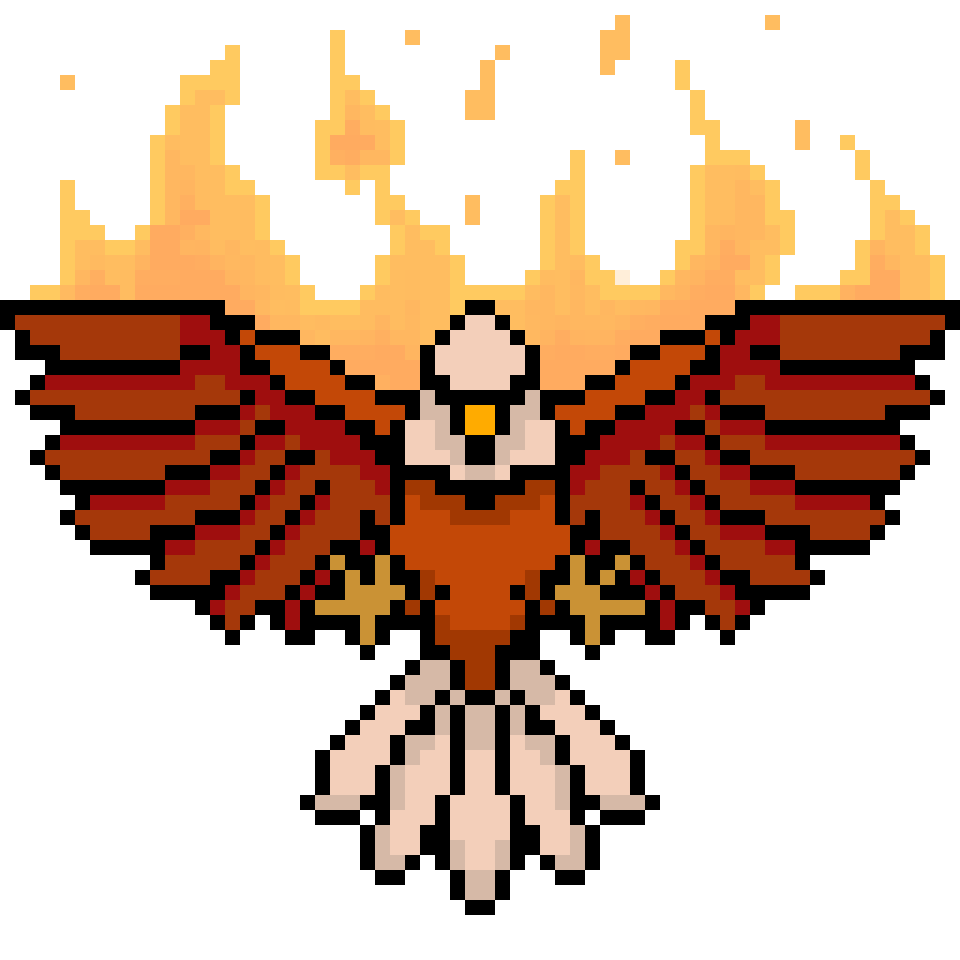
\includegraphics[width=.8\textwidth]{img/sprites/aigle_feu.png}
\end{minipage}

\begin{minipage}{.75\textwidth}
    \paragraph{Aigle de gel}\label{sec:gel}
    L'aigle de gel est un aigle persistant qui empêche la rotation de toutes les
    cases dans son rayon d'action. % footnote : ils fuient, ils meurent !
    Il empêche aussi bien les rotations des deux joueurs que les rotations des
    aigles météores.
\end{minipage}
\begin{minipage}{.2\textwidth}
    \centering
    
\includegraphics[width=.8\textwidth]{img/sprites/aigle_glace.png}
\end{minipage}

\begin{minipage}{.75\textwidth}
    \paragraph{Aigle de mort}
    L'aigle de mort est un aigle éphémère qui, une fois activé, fait disparaitre
    tous les aigles dans son rayon d'action
    \footnote{Aucun aigle n'est maltraité pendant la durée de la partie.
    Contrairement à ce que son nom pourrait faire penser, l'aigle de mort fait
    simplement \textbf{fuir} les autres aigles en dehors de la carte.}.
    Il peut donc faire disparaitre les aigles adverses, mais aussi vos propres
    aigles et les aigles sauvages.
    
    Un aigle de mort ne peut cependant pas faire fuir un aigle qui n'a pas encore
    éclos.
\end{minipage}
\begin{minipage}{.2\textwidth}
    \centering
    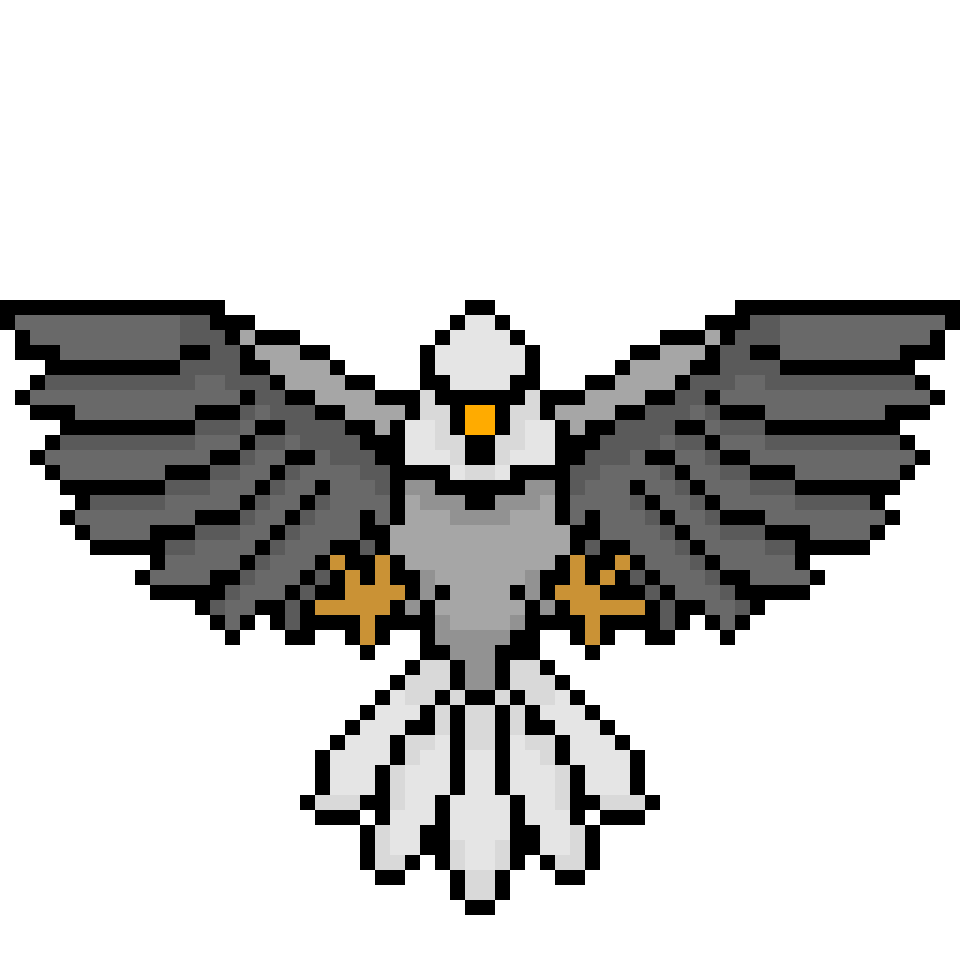
\includegraphics[width=.8\textwidth]{img/sprites/aigle_peur.png}
\end{minipage}

\begin{table}[h]
    \centering
    \begin{tabular}{r|l|l}
        Aigle   & Longévité & Effet                                                   \\
        \hline
        Vie     & Éphémère  & Rajoute des points d'actions pour le tour actuel        \\
        Météore & Éphémère  & Tourne d'un demi-tour les cases dans son rayon d'action \\
        Feu     & Persistant & Multiplie le gain d'un emplacement                      \\
        Gel     & Persistant & Empêche les rotations dans son rayon d'action            \\
        Mort    & Éphémère  & Fait fuir les aigles dans son rayon d'action            \\
    \end{tabular}
\end{table}

\newpage
\section{Règles}
\paragraph{Début d'une partie}
Chaque joueur commence la partie avec en sa possession un unique village,
sans aucun aigle.
Une partie est composée de $\dfrac{\mathtt{NB\_TOURS}}2$ rounds, chaque round
étant divisé en deux tours, un tour par joueur.

Avant le commencement du premier tour, la fonction \texttt{partie\_init}
de votre champion est appelée.
% Capture

\paragraph{Déroulement d'un tour}
Au commencement de chaque tour, s'il s'agit de votre tour, la fonction
\texttt{jouer\_tour} de votre champion est appelée.
Vous disposerez alors de \texttt{TOUR\_POINTS\_ACTION} points d'actions
pour effectuer vos actions.
Vous pouvez alors, autant de fois que vous le souhaitez~:
\begin{itemize}
    \item
        Tourner une case arbitraire d'un quart de tour dans le sens
        trigonométrique, tant que vous disposez de suffisamment de points
        d'actions.
        Si la case tournée borde un emplacement du territoire adverse, alors
        cette action demande \texttt{COUT\_ROTATION\_ENNEMI} points d'action,
        sinon l'action demande \texttt{COUT\_ROTATION\_STANDARD} points
        d'action.
        Vous ne pouvez pas tourner un village, ni tourner une case étant
        gelée par un aigle de gel.
    \item
        Déplacer un aigle vous appartenant sur un emplacement arbitraire.
        Cela ne coûte aucun point d'action et peut être réalisé librement
        autant de fois que souhaité.
        Plusieurs aigles peuvent se situer sur le même emplacement.
    \item
        Activer l'effet d'un aigle éphémère qui vous appartient.
        L'aigle ainsi utilisé disparait alors.
        Cela ne demande aucun point d'action, vous pouvez activer autant
        d'aigles que vous souhaitez pendant un même tour.
        L'effet d'un aigle permanent est toujours actif.
\end{itemize}

\paragraph{Score}
À la fin de chaque tour, la somme des gains de chaque
île dans votre territoire est ajouté à votre score.
Un aigle de feu (vous appartenant ou non) permet de multiplier le gain d'un
emplacement.
Au dernier tour, cette somme est multipliée par
\texttt{MULTIPLICATEUR\_DERNIER\_TOUR}.

\paragraph{Fin de jeu}
À la fin du dernier tour, la partie prend fin
et la fonction \texttt{partie\_fin} de votre champion est appelée.
Le joueur ayant le plus grand score est déclaré vainqueur de la partie.
